\documentclass[11pt,a4paper]{kth-mag}

% \usepackage{fontspec}
\usepackage[backend=bibtex]{biblatex}
\usepackage{pdflscape}
\usepackage{rotating}
% \usepackage[top=1cm]{geometry}
\usepackage{subfig}
\usepackage{amsmath}
\usepackage{hyperref}
\usepackage[ruled,vlined]{algorithm2e}
\usepackage{graphicx}
\usepackage{moreverb}
\usepackage{longtable}
\usepackage{xhfill}
\renewcommand{\textquotedbl}{\texttt{"}}
\newcommand{\ditto}[1][.4pt]{\xrfill{#1}~\textquotedbl~\xrfill{#1}}
%\usepackage[toc,page]{appendix}
\setcounter{tocdepth}{3}
\setcounter{secnumdepth}{3}
% \defaultfontfeatures{Mapping=tex-text}
% \setromanfont[Ligatures={Common},Numbers={Lining}]{Linux Libertine}

\bibliography{report.bib}

\author{Michal Staniaszek}
\title{A System for Object Query in Point Clouds Using Feature-Feature Matching}

\begin{document}
\maketitle
\begin{abstract}
  In this report, we will describe our implementation of a system for retrieving
  instances of objects using feature based matching techniques. We use point
  cloud data gathered using RGB-D sensors in an office environment over a period
  of approximately a month. Some preprocessing steps are applied to the data to
  reduce the size of the clouds and use basic RANSAC-based plane segmentation to
  remove parts which we believe will not contain any objects. Using locations
  determined by one of several possible interest point selection methods, one of
  a number of possible types of features is extracted. Using a nearest neighbour
  approach, these features, are compared to a corresponding set extracted from a
  cloud representing a query object. Results from this comparison are used to
  vote for the position of the object in a 3D grid overlaid on the room cloud.
  We then cluster these votes and rank the clusters. The centroid of each of the
  clusters is used to extract a region from the room cloud which, in the ideal
  case, corresponds to the object that was passed to the system.

  We perform an experimental evaluation of the system using various parameter
  settings in order to investigate computation time and other factors affecting
  the usability of the system.
\end{abstract}
\tableofcontents
\chapter{Introduction}
Having a large amount of data is in most cases a good thing. Data, in an
abstract sense, is the driving force behind the actions of every living thing,
and as such holds great power. However, in order to make use of data, it is
necessary to have some way of interacting with it in a useful way, and further
processing it. While technologies for storing and interacting with data have
been around for millennia, for the most part they were inconvenient and
cumbersome. Writing allowed practically lossless transfer of information between
generations, and is no doubt one of the most important inventions in the history
of humanity. That being said, books are quite limited, especially when one wants
to investigate a specific topic. Libraries are partial solutions to the problem,
but most libraries don't possess all books in existence, and while indexes exist
for a reason, it is still not easy to find what one is looking for.

With the internet and the immense amount of data available to its users, this
problem of finding what one is looking for has been compounded, and good ways of
getting around the problem have launched one of the most successful companies in
history. At first, listing all of the early internet to create a database was a
realistic proposition, and for some time this was a satisfactory solution.
However, as the number of accessible data on the internet grew, the system
became gradually more impractical. It could take minutes or even hours to get a
result for a query, and the trawling of content caused network slowdowns
\cite{firstsearch,archieabout,bowman1993research}. Subsequent work in the area
led to the development of search engines which were able to search for words in
pages, and various innovations led this to become the very effective way of
searching that we know today \cite{brin1998anatomy,pinkerton1994finding}.

While images have been on the internet since the early days, in recent years the
advent of affordable digital cameras and the ubiquity of mobile phone cameras
has led to hundreds of thousands of photographs being uploaded to the internet
every minute \cite{fbipo,photosminute}. At its most basic, image search utilises
the same techniques as text search, with information being extracted from
metadata like tags, descriptions and keywords \cite{jing2008pagerank}. More
recently, reverse image search has become more popular, allowing users to find
similar images to an example by extracting information from textures and trying
to find other images which contain similar information \cite{lew2006content}.
There is still much information present in images that cannot currently be
extracted and represented using image processing techniques, and this is an
active research area.

An emerging method of data storage that will need to be searchable in the near
future is 3D models and point clouds. 3D models have been used for a long time
in computer games, medical imaging, and animation. More recently, developments
in 3D printing have led to a growing number of websites which distribute models
to use for printing \cite{3dprintlist}. For many years these sorts of models
have been created using CAD programs, or in the case of object scanning,
expensive time-of-flight cameras. The release of the Microsoft Kinect in late
2010 marked a turning point in the realm of 3D image processing, creating an
affordable and effective method of gathering 3D data. Many research groups
quickly purchased the hardware, and much work has been done in the area since. A
3D equivalent of the popular 2D image processing library OpenCV quickly came
into existence for use with point clouds, as the data which comes from such 3D
sensors is known \cite{opencv, pcl}.

In this report, we will describe our approach the problem of retrieving from a
data set objects that are similar to some object that we have provided, which we
will call object query. In essence, we need to extract information from the data
set and the objects that we are interested in which describes their properties
in such a way that we can compare the descriptions to see if there are any
similarities that imply the presence of an object in the data set. While the
data set could be anything, in our particular case we have data from a project
which studies long-term robot operation in office environments. The data set
contains point clouds of a single office taken from the same position over a period
of approximately a month. Some objects in the data set have also been labelled,
so there is information about the positions of objects in the clouds.

While this project is not aiming to perform a specific task on an actual robotic
system, within this context there are applications to which an object query
system could be applied. Given a data set over long periods of time with clouds
taken at various locations, the system could be used to track the motion of
objects over time, and to provide information about where an object is likely to
be at a certain time. One potential application is to help people find objects
that have been misplaced.

The project will focus in particular on the implementation of a system which can
perform object query. It will evaluate a number of standard methods for
describing objects, and finding parts of objects that are particularly
discriminative. While it is possible to describe objects as a whole, we will
investigate the efficacy of using descriptions of small parts of the object to
retrieve matches from the data set. Matches are found by comparing these
descriptions, which are generally vectors of scalar values, to each other, and
finding those which have the most similar values. This approach is called
feature matching.

While the use of descriptors is the basis for the majority of systems for object
retrieval, in most cases there are several additional layers applied on top of
the basic feature-feature matching in the lower levels. This often includes
costly pre-segmentation of the input data, where it is necessary to determine
what parts of the clouds are actually objects in order to create a description
of them to use later. If the data is labelled in some way, this can be
relatively easy to achieve, but we are interested in querying data which has no
labels at all. As a result, we would like to investigate the effectiveness of
using a very simple approach to the problem which does not required complex
reasoning about the nature of objects.

In chapter~\ref{chap:bg}, we explain some concepts that are important to
understand the work, provide background information on relevant parts of the
image processing literature, and attempt to introduce the reader to previous
work in similar areas. The preprocessing steps that we apply to clouds are
described in chapter~\ref{chap:preprocess}. Brief descriptions of the interest
points and descriptors that we use are given in chapters~\ref{chap:interest} and
\ref{chap:descriptors} along with some explanation as to why we wish to use
these methods. Chapter~\ref{chap:query} is the final chapter describing our
system, wherein we discuss our approach to using descriptors to retrieve
objects. Our experimental setup and the results of the experiments are described
in chapter~\ref{chap:exp}. We compare the quality of retrieval when different
methods are used, and also investigate the time taken by the system under
varying parameter settings. Finally, we summarise the system and our results in
chapter~\ref{chap:conc}.
\chapter{Background}
\label{chap:bg}
In this chapter we will introduce some key ideas relating to the project, and
papers which are related to what we are interested in doing. While some of the
techniques mentioned here are not directly used in the implementation of our
system, they can be useful for context, or to give examples of different ways of
approaching problems in this area. We discuss methods of finding interesting
regions in image and point cloud data, and how these regions can be represented
using descriptors, along with some methods for storing descriptors in ways that
make it easy and efficient to find similarities.

\section{Segmentation}
Segmentation encompasses techniques for splitting an image or a point cloud into
different parts, or grouping similar parts --- this is essentially two sides of
the same coin. In terms of images, segmentation might be used to try to find
background and foreground pixels, or for point clouds, to separate objects from
the surfaces on which they are resting. There are many different types of
methods in the area, which approach the problem from different starting points.

\begin{figure}
  \centerline{
    \subfloat[Superpixels size 64, 256 and 1024 computed using SLIC \cite{achanta2012slic}]{
      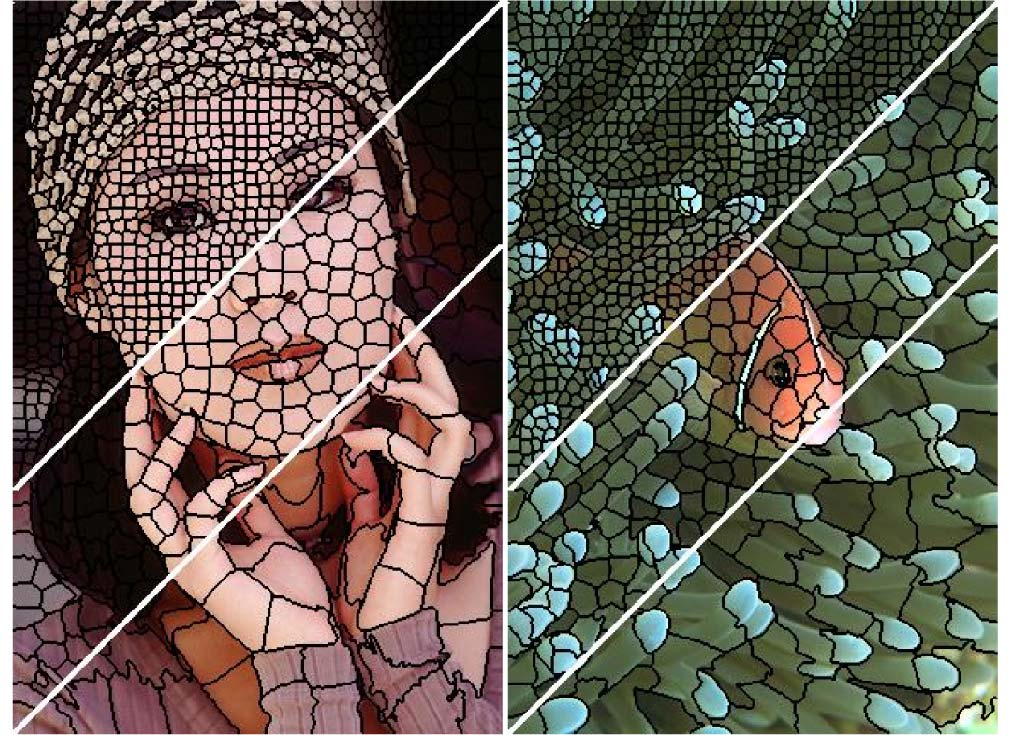
\includegraphics[height=0.3\textheight]{images/slic}
    }
    \subfloat[Supervoxel oversegmentation \cite{papon2013voxel}]{
      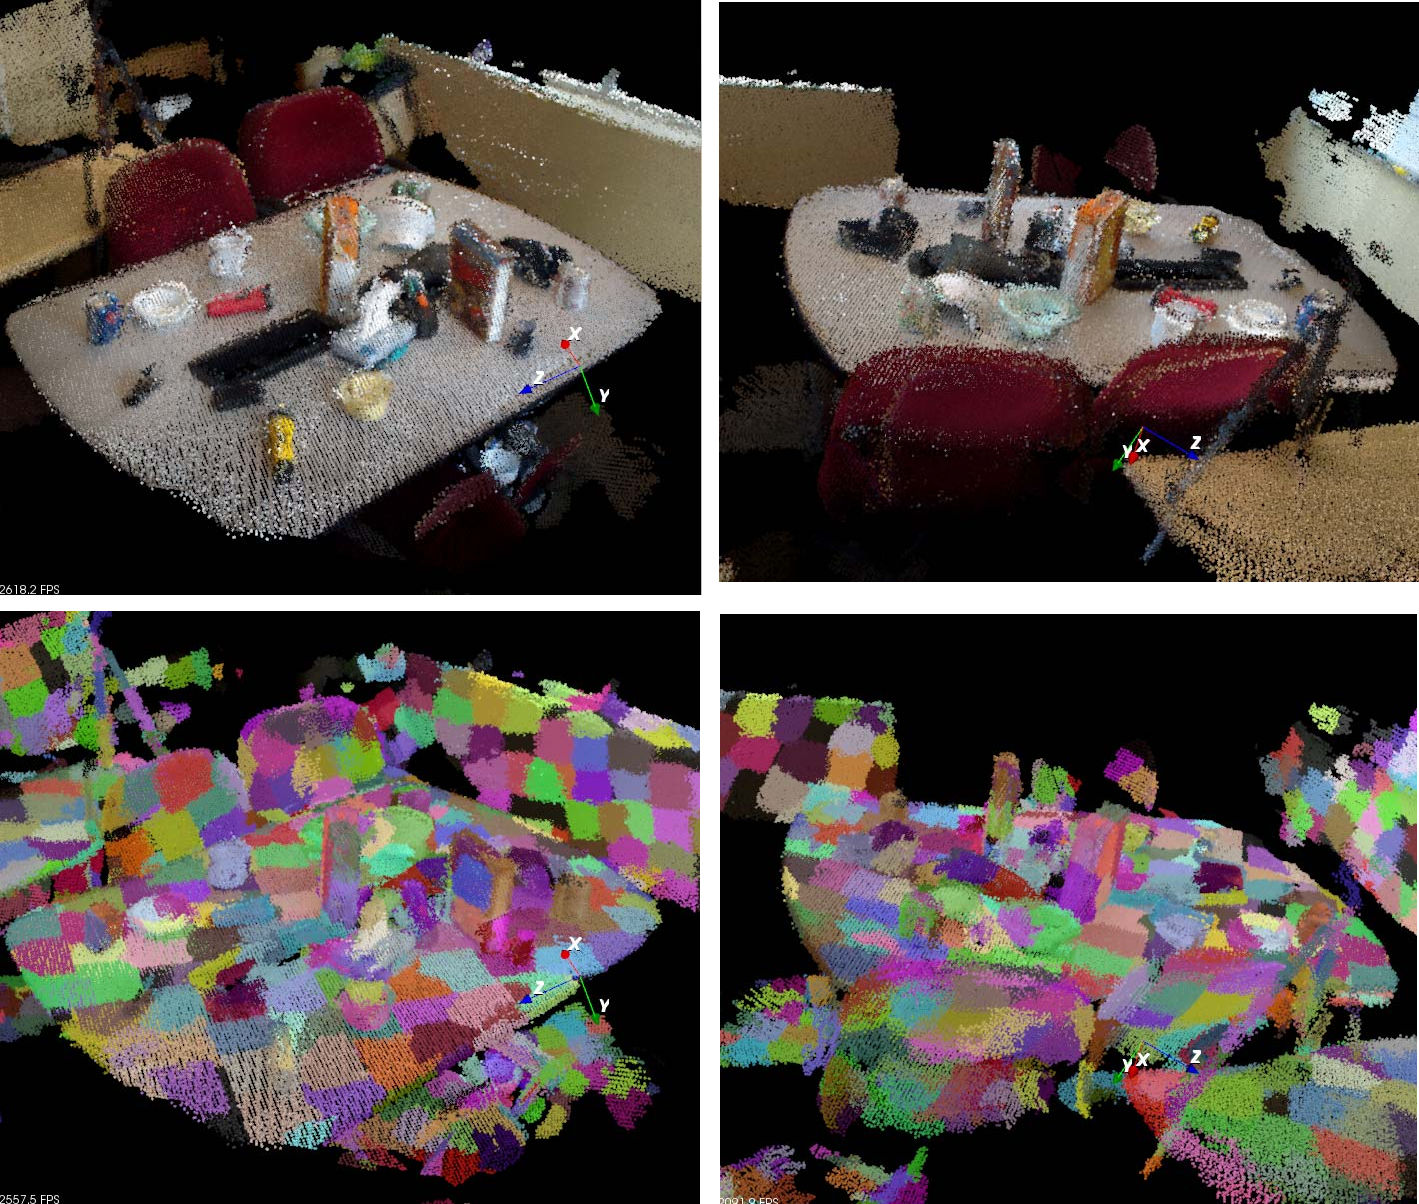
\includegraphics[height=0.3\textheight]{images/supervoxel_comb}
    }
  }
    \caption{Examples of 2D and 3D superpixel segmentations}
    \label{fig:meanshift}
\end{figure}

Superpixel clustering is the most common technique used for segmenting images.
The intent is to create regions in which all pixels have some sort of meaningful
relationship. Graph based algorithms treat pixels as nodes in a graph, where the
weights on edges between nodes are related to the similarity between the
connected pixels --- intensity, proximity and so on \cite{achanta2012slic}. The
most simple method is to use a threshold on the edge weights to create
superpixels. Fulkerson et al. use superpixel methods to identify object classes
in images \cite{fulkerson2009class}. An algorithm which applies the idea of
superpixels to point clouds to create supervoxels (3D pixels) has also been
developed \cite{papon2013voxel}.

Gradient ascent based algorithms iteratively improve clusters until some
criterion for convergence is reached \cite{achanta2012slic}. Popularised by
Comaniciu~\cite{comaniciu2002mean}, mean shift was first introduced by
Fukunaga~\cite{fukunaga1975estimation} in 1975, and rediscovered by
Cheng~\cite{cheng1995mean} in 1995. The technique finds stationary points in a
density estimate of the feature space, for example pixel RGB values, and uses
those points to define regions in the space by allocating pixels to them. One
common way of computing a density estimate is to place Gaussians at the location
of each pixel, and then to sum the values of all the Gaussians over the entire
space. Pixels which follow the gradient of the density to the same stationary
point are part of the same segment. An example can be seen in
Figure~\ref{fig:meanshift}.
\begin{figure}[t]
  \centering
  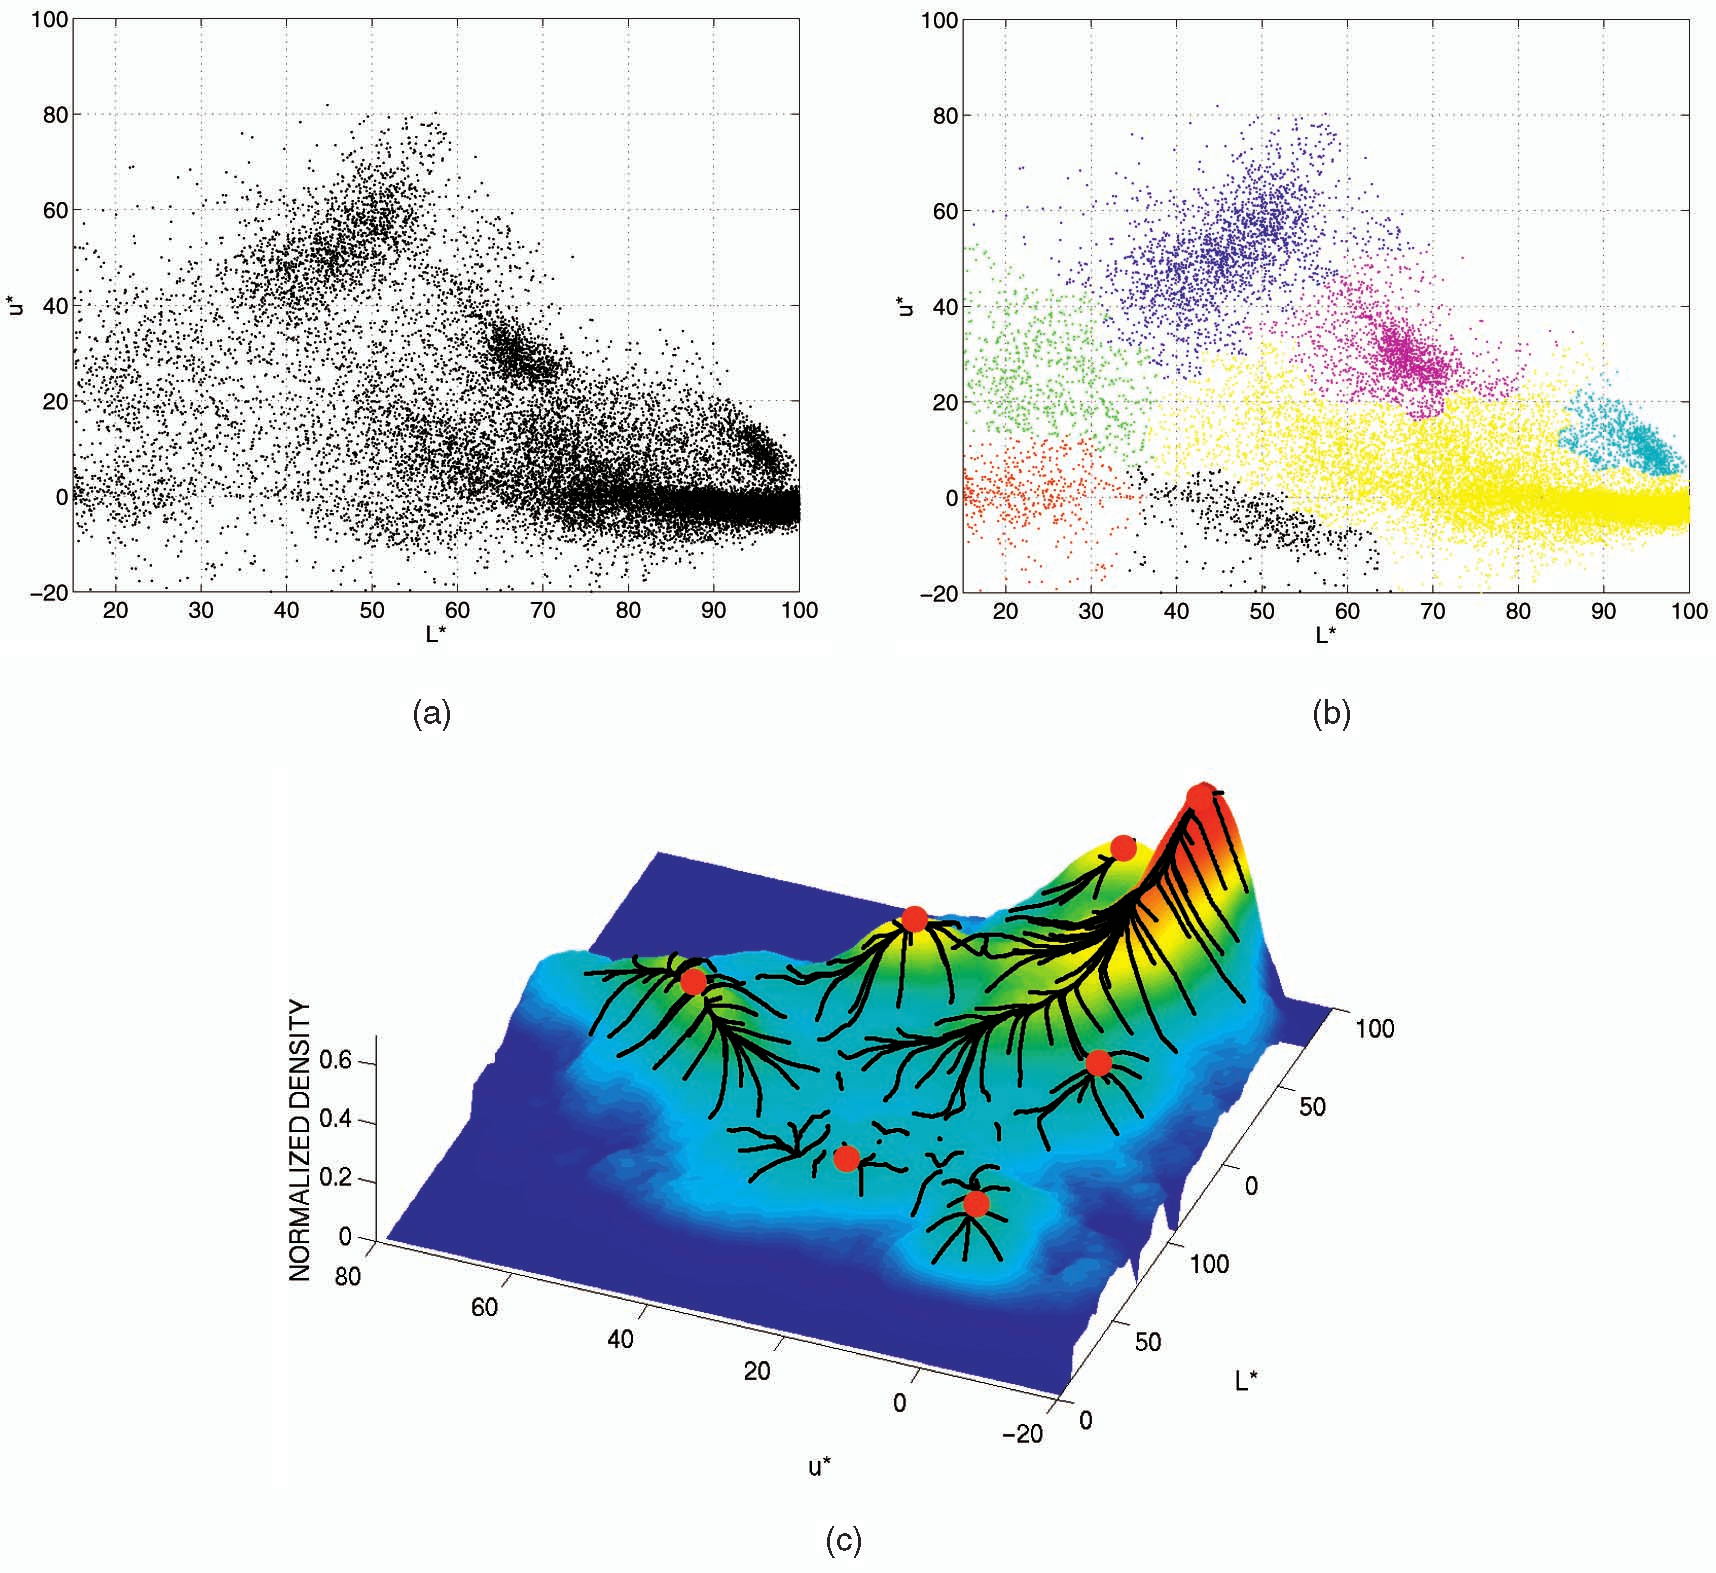
\includegraphics[width=\textwidth]{images/meanshift}
  \caption{Visualisation of mean shift \cite{comaniciu2002mean}. a) First two
    components of image pixels in LUV space. b) Decomposition found by running
    mean shift. c) Trajectories of mean shift over the density estimate.}
  \label{fig:meanshift}
\end{figure}


Random Sample Consensus (RANSAC) is a technique which uses shape models to find
ideal models in noisy data. Points in the data set are randomly sampled, and
used to construct a shape. For example, in the case of a line, two points are
sampled, and define the line. Distances from points in the data set to the model
defined by the randomly sampled points are then computed to find points which
are inliers to the model. This number is stored, and the process repeated a
number of times. At the end of the process, the model with the largest number of
inliers is returned \cite{fischler1981random}. RANSAC can be applied to
segmentation tasks by using it to find planes, cylinders, spheres and so on in
point clouds. In the case of planes this is particularly useful, as they are
usually not part of objects of interest, mostly making up walls, floors or
surfaces on which interesting objects rest. By removing the points corresponding
to these uninteresting surfaces, it should be possible to work only with parts
of clouds that contain objects of interest.

Several extensions to RANSAC have been proposed. Maximum Likelihood Estimation
Sample Consensus (MLESAC) chooses a solution that maximises the likelihood of
the model instead of just the number of inliers \cite{torr2000mlesac}.
M-estimator Sample Consensus (MSAC) uses a different cost function to the
original implementation, additionally scoring the inliers depending on how well
they fit the data \cite{torr2000mlesac}. The Progressive Sample Consensus
(PROSAC) uses prior information about the likelihood of input data being an
inlier or an outlier to limit the sampling pool and greatly reduce computation
cost \cite{chum2005matching}.


\section{Interest Points and Saliency}
Sipiran and Bustos extend the popular Harris detector \cite{harris1988combined}
to 3D \cite{sipiran2011harris}. Knopp et al. extend the SURF detector to 3D
\cite{knopp2010hough}.

Shilane and Funkhouser introduce a distinctiveness measure over classes of
meshed objects \cite{shilane2007distinctive}.

A multi-scale signature defined by the heat diffusion properties of an object
called the Heat Kernel Signature (HKS) \cite{sun2009concise} is used in
\cite{ovsjanikov2009shape} to retrieve shapes.

\cite{zhong2009intrinsic}

\cite{smith1997susan} extended to 3d by adding normal direction variation to
intensity variation

\section{Descriptors}
The problem of describing regions of an image in a compact and useful manner has
been studied for a long time in the computer vision community. For any given
point in an image, we would like to create a description which can be used to
represent the region around the point in some way. This descriptor, or feature,
can then be compared to other descriptors to see if there is some similarity. If
the similarity is within a given threshold, then we can assume that the points
represented by the two descriptors come from the same object, or represent the
same thing in both images. Thus, it is important to create features which are
distinct for different regions. In addition, since objects move around and can
be seen from different sides, or in different lights, an attractive property of
descriptors is to give similar results for the same region which has been
transformed in some way. In practice, this is quite difficult to achieve.
\subsection{2D}
While 2D descriptors are not directly usable on point clouds, the ideas that
they use to give effective results can be transferred over to use for 3D
description.

The Laplacian of Gaussians was introduced by Lindeberg, and uses derivatives
combined with some other techniques to select interest points.
\cite{lindeberg1998feature}. This paper also introduces the concept of automatic
scale selection for feature detection, which has played an important part in the
field since then. The scale of features can be investigated by blurring an image
using a Gaussian kernel --- higher standard deviation blurs the image more,
resulting in the removal of small scale features.

Even today the Scale Invariant Feature Transform (SIFT) is among the most
popular descriptors for 2D images. It is invariant to scale and rotation, and is
robust to some variation in affine distortion, viewpoint and illumination, and
is distinctive, allowing for correct matching of single features in large
databases. There are several stages of computation. Extrema are found in
different scales to find points invariant to scale and orientation. Keypoints
are selected at the extrema based on their stability. Image gradients at the
keypoint are used to define its orientation for future computations. The image
gradients are then transformed into a local descriptor vector with length 128
\cite{lowe2004distinctive}.

Mikolajczyk and Schmid~\cite{mikolajczyk2004scale} introduce the Harris-Laplace
detector which is an improvement on SIFT \cite{lowe2004distinctive} and the
Laplacian of Gaussians \cite{lindeberg1998feature} in the sense that it is able
to deal with affine transformations. They do not, however, introduce a new type
of descriptor to go with the point selection. 

Speeded-Up Robust Features (SURF) is a more recent descriptor which can be
computed and compared much faster than most other descriptors. It makes use of
integral images, which replace pixels in an image or image patch with a
cumulative sum of the pixel intensities over the rows and columns. This allows
for fast computation of pixel intensities in an area of the image. SURF takes
some ideas from SIFT, using the spatial distribution of gradients as a
descriptor, but integrates over the gradients instead of using individual
values, which makes it more robust to noise. The resulting descriptor is a 64
element vector, which means that it is also faster to compare than SIFT
\cite{bay2008speeded}.

\subsection{3D}
One early descriptor which remains popular is the spin image. The descriptor is
generated from a mesh model at oriented points with a surface normal. A plane
intersecting the normal with a certain width and height is rotated around the
normal, forming a cylinder. The plane is separated into bins. The bins
accumulate the number of points which pass through a certain bin during the
rotation. The resulting 2D image is the descriptor. By varying the width of the
plane the region which defines the descriptor can be modified. A small width
will give a local descriptor, while a large width will give a descriptor for the
whole image \cite{johnson1997spin,johnson1999using}. Figure~\ref{fig:spinimg}
shows a visualisation of how the image is generated.

\begin{figure}
  \centering
  \subfloat{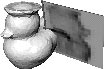
\includegraphics[width=0.11\textwidth]{images/spin1}}
  \subfloat{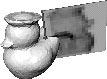
\includegraphics[width=0.11\textwidth]{images/spin2}}
  \subfloat{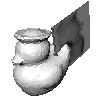
\includegraphics[width=0.11\textwidth]{images/spin3}}
  \subfloat{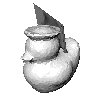
\includegraphics[width=0.11\textwidth]{images/spin4}}
  \subfloat{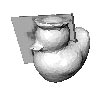
\includegraphics[width=0.11\textwidth]{images/spin5}}
  \subfloat{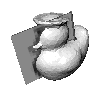
\includegraphics[width=0.11\textwidth]{images/spin6}}
  \subfloat{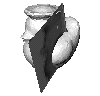
\includegraphics[width=0.11\textwidth]{images/spin7}}
  \subfloat{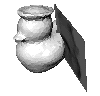
\includegraphics[width=0.11\textwidth]{images/spin8}}
  \caption{Frames from construction of a spin image \cite{johnson1997spin}. The
    image plane spins around the oriented point normal and accumulates points.}
  \label{fig:spinimg}
\end{figure}

The Ensemble of Shape Functions (ESF) descriptor introduced in
\cite{wohlkinger2011ensemble} by Wohlkinger and Vincze combines the Shape
Distribution approach introduced by \cite{osada2002shape} along with some
extensions proposed in \cite{ip2002using}. It also makes use of their
voxel-based distance measure from \cite{wohlkinger2011shapedist}. Pairs or triples of
points are sampled from segmented partial clouds of objects, and histograms are
created by extracting information such as distance, angle, ratios, and whether
points are inside or outside (or a mix) of the model. See
Figure~\ref{fig:wohlESF}.

The Point Feature Histogram (PFH) was introduced by Rusu et al. in
\cite{rusu2008persistent}. It creates descriptors based on the angles between a
point on a surface and $k$ points close to it. The Fast Point Feature Histogram
(FPFH) improved the speed of computation, and allowed the use of the descriptor
in real time \cite{rusu2009fast}. The Viewpoint Feature Histogram (VFH) extended
the FPFH by adding viewpoint information to the histogram by computing
statistics of surface normals relative to the viewpoint \cite{rusu2010fast}. It
also improved the speed of the FPFH. The clustered version (CVFH) further
improved the viewpoint technique by mitigating the effect of missing parts and
extending it to facilitate estimation of the rotation of objects \cite{aldoma2011cad}.

Bo et al. develop the kernel descriptor initially created for RGB images for use
on depth images and point clouds. The kernels are used to describe size, shape
and edge features. Local features are combined to object-level features . Kernel
descriptors avoid the need to quantise attributes. Similarity is instead defined
by a match kernel \cite{bo2010kernel}, which improves recognition accuracy
\cite{bo2011depth}.

The point pair feature describes the relation between two oriented points on a
model. This means that it does not depend so much on the quality and resolution
of the model data. The model is described by grouping the point pair features of
the model, providing a global distribution of all the features on the model
surface \cite{drost2010model}.

\begin{figure}
  \centering
  \subfloat[3DSC \cite{frome2004recognizing}]{
    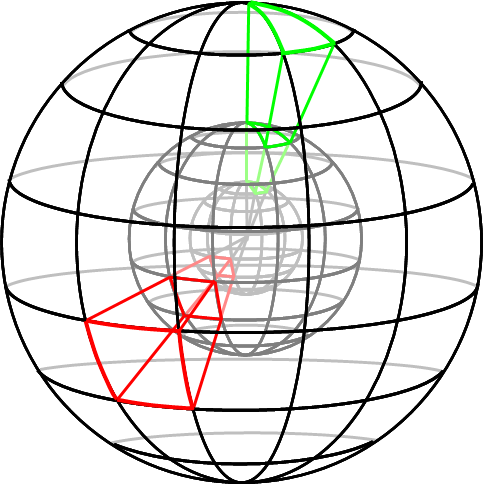
\includegraphics[width=0.24\textwidth]{images/3dsc}
    \label{fig:3dsc}
  }
  \subfloat[SHOT \cite{tombari2010unique}]{
    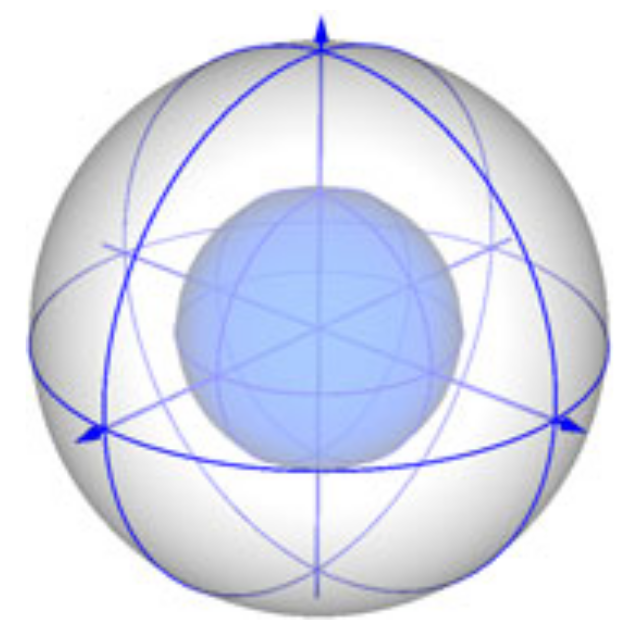
\includegraphics[width=0.24\textwidth]{images/shot}
    \label{fig:shot}
  }
  \subfloat[Context Shape \cite{shentu2008context}]{
    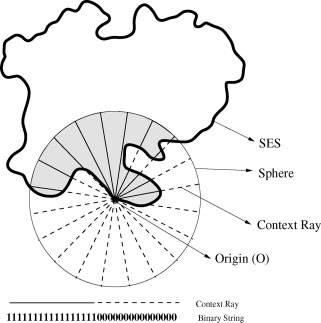
\includegraphics[width=0.24\textwidth]{images/contextshape}
    \label{fig:contextshape}
  }
  \subfloat[Integral Volume \cite{gelfand2005robust}]{
    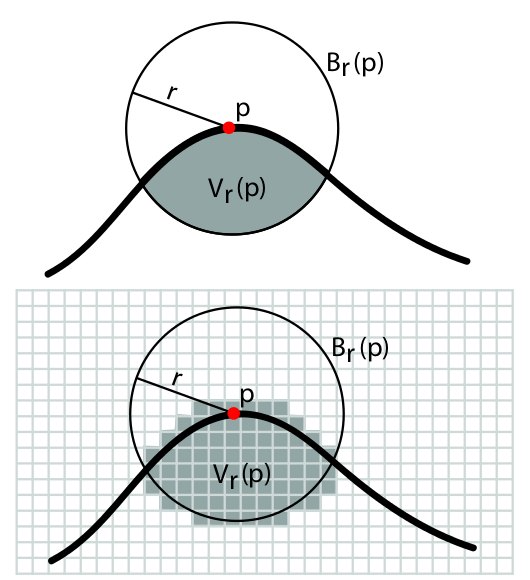
\includegraphics[width=0.24\textwidth]{images/volint}
    \label{fig:volint}
  }
  \caption{Visualisation of spherical descriptors.}
  \label{fig:descexample}
\end{figure}

3D Shape Context (3DSC) is an extension of the original Shape Context descriptor
for 2D images \cite{belongie2002shape}. A sphere is placed at a point, and its
``top'' is oriented to match the direction of the normal at the point. Bins are
created within the sphere by equally spaced boundaries in the azimuth and
elevation, and logarithmically spaced boundaries in the radial dimension (Figure~\ref{fig:3dsc}). The
logarithmic spacing means that shape distortions far from the basis point have
less effect on the descriptor. Each bin accumulates a weighted count based on
the volume of the bin and local point density \cite{frome2004recognizing}. 3DSC
does not compute a local reference frame --- the vector of the azimuth is chosen
randomly, and subdivisions computed from that. This means that a number of
descriptors equal to the number of azimuth divisions need to be computed and
stored in order to compensate, and the matching process is complicated as a
result. The Unique Shape Context (USC) solves this problem by defining a local
reference frame and using the directions of that reference frame to subdivide
the sphere \cite{tombari2010uniquesc}.

The Signature of Histograms of Orientations (SHOT) descriptor improves on 3DSC
by taking inspiration from SIFT and making extensive use of histograms. The
sphere is split into 32 volumes: 8 azimuth regions, 2 elevation and 2 radial
(Figure~\ref{fig:shot}). A local histogram is computed in each of the regions,
using the angle between the normal of points and the feature point. The local
histograms are then combined to form the final descriptor
\cite{tombari2010unique}. The authors also extend the descriptor to include
colour (COLORSHOT) \cite{tombari2011combined}.

The Rotation Invariant Feature Transform (RIFT) is a generalisation of SIFT. Using
intensity values computed at each point from the RGB values, a gradient is
computed. Concentric rings are placed around the initial point, and a histogram
of the gradient orientations is created for points within each ring. The
orientation of the gradient is computed relative to the line from the central
point so that the descriptor is rotation invariant. The descriptor is 2D --- one
dimension is the distance, the other the gradient angle. The distance between
two descriptors is measured using the earth mover's distance (EMD), which is a
measure of the distance between two probability distributions
\cite{lazebnik2005sparse}.

Multi-scale descriptors are useful as they can be used to characterise regions
of varying size. Cipriano et al. introduce such a descriptor for use on meshes
\cite{cipriano2009multi}. It captures the statistics of the shape of the
neighbourhood of a vertex by fitting a quadratic surface to it. Vertices in the
region are weighted based on distance from an initial vertex, and a plane is
constructed using a weighted average of the face normals. The parameters of the
quadratic are then used to find its principle curvatures, which make up the
descriptor.

Work in protein-protein docking also uses 3D descriptors to help with
simulations of an otherwise lengthy and complex process. The Surface Histogram
is introduced by Gu et al. \cite{gu2012surface}, and uses the local geometry
around two points with specific normals on the surface of a protein. A
coordinate system is defined by the two points and the line between them, and a
rectangular voxel grid is defined around the points. The grid is then marked in
locations where the surface crosses the grid, and a 2D image is constructed by
squashing the data onto one of the axes. The descriptor is designed to
immediately give a potential pose for the docking.

Another example of a shape descriptor from biology is the Context Shape
\cite{shentu2008context}. A sphere is centred on a point, and rays are projected
from this point to points evenly distributed on the surface of the sphere (Figure~\ref{fig:contextshape}). Each
of the rays is divided into segments, with a binary value associated with each
segment depending on whether the segment is inside or outside the protein. To
compare the descriptor, a rotation is applied to match the rays, and a volume of
overlap is computed based on matching bits in the rays.
 
\begin{figure}
  \centering
  \subfloat[]{
    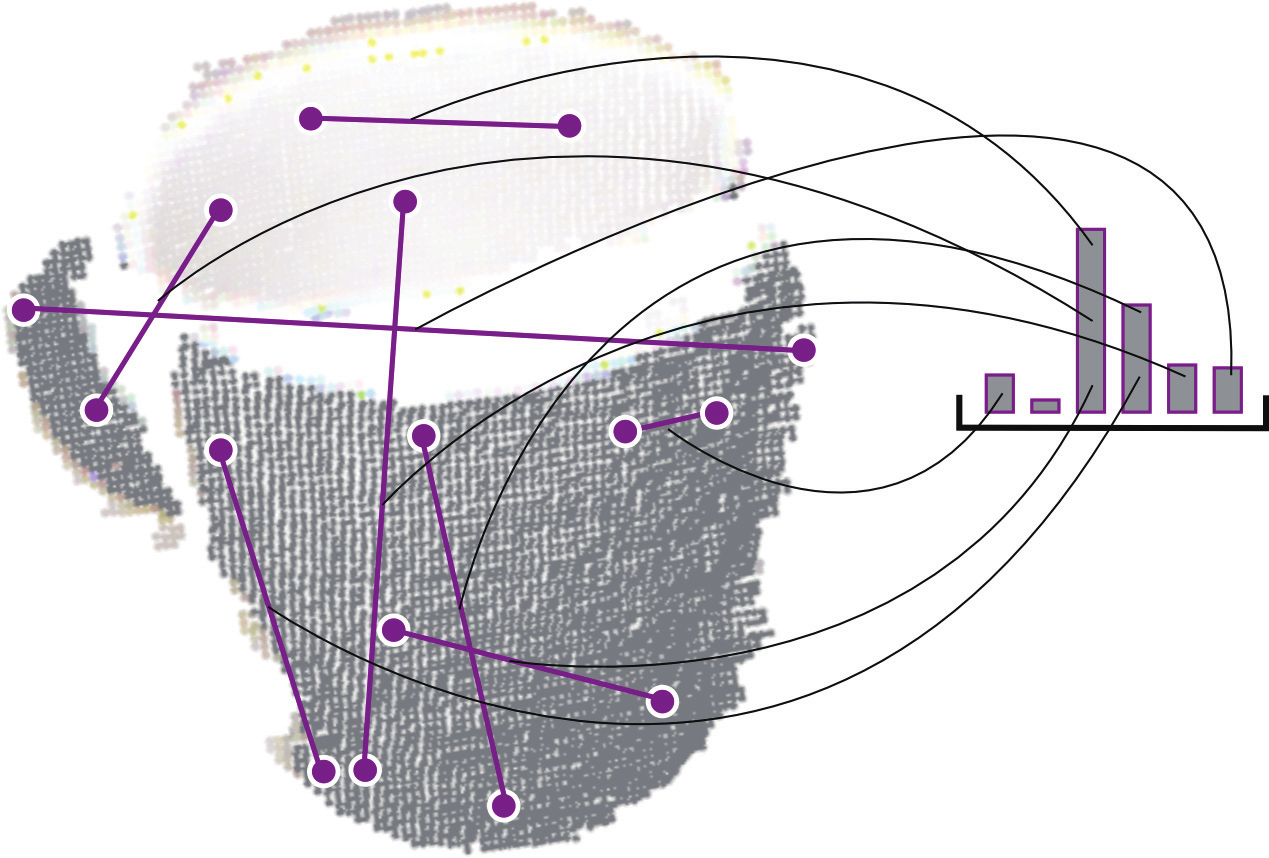
\includegraphics[width=0.23\textwidth]{images/wohl_d2}
  }
  \subfloat[]{
    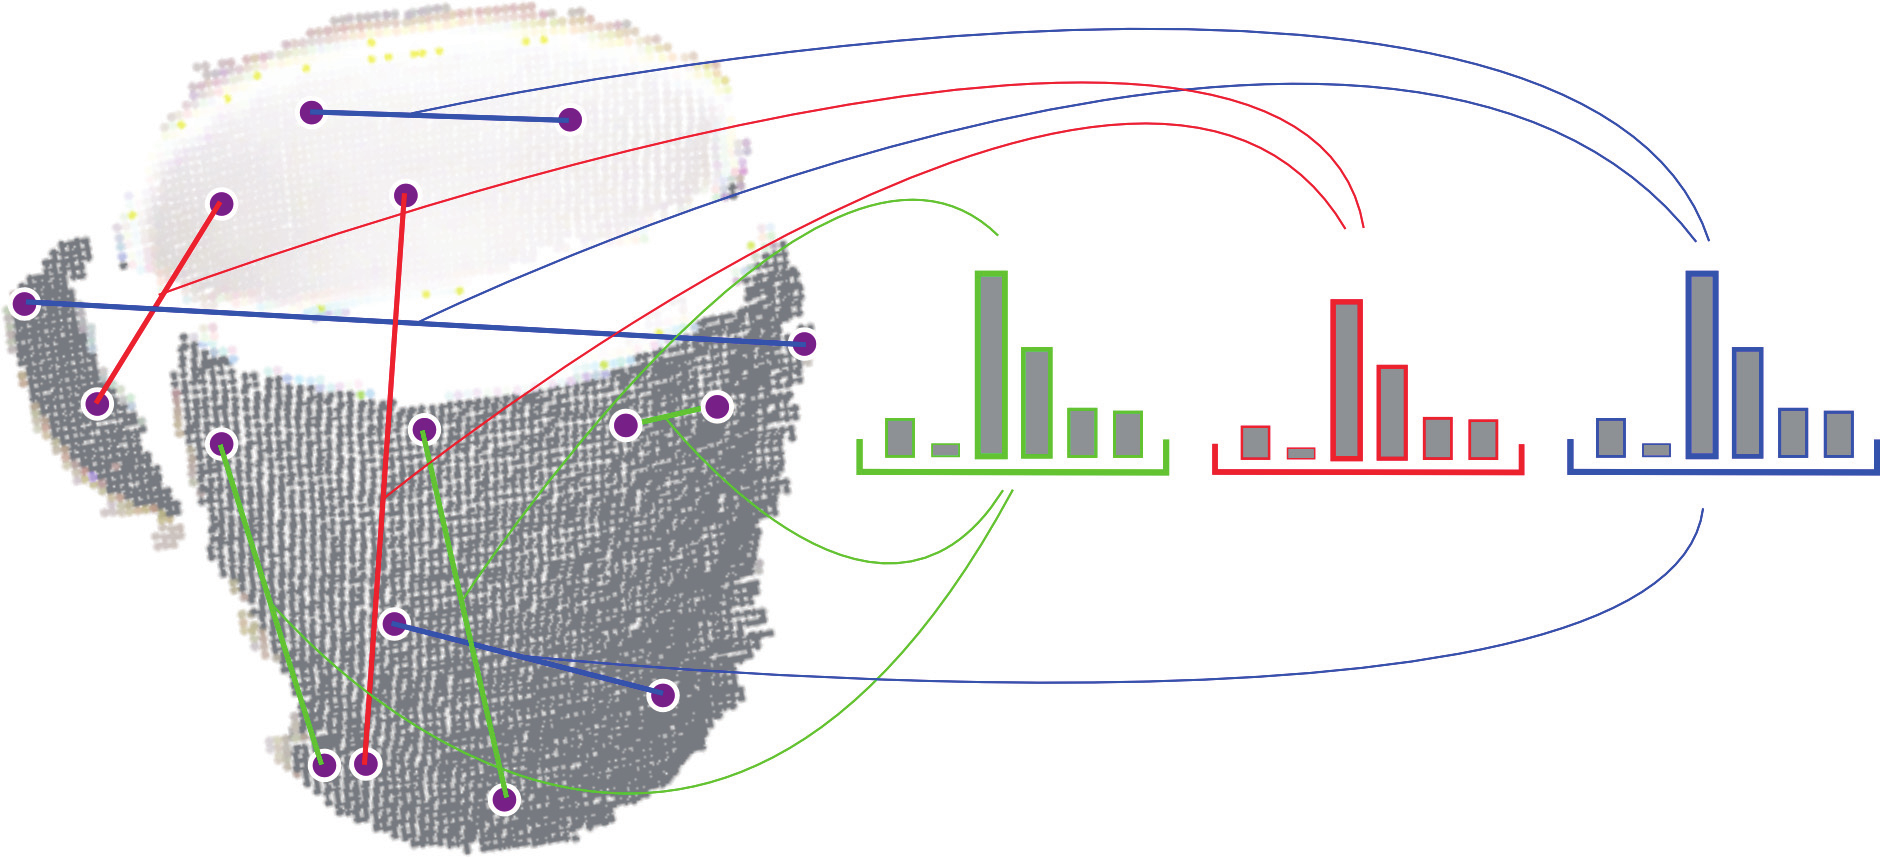
\includegraphics[width=0.23\textwidth]{images/wohl_onoff}
  }
  \subfloat[]{
    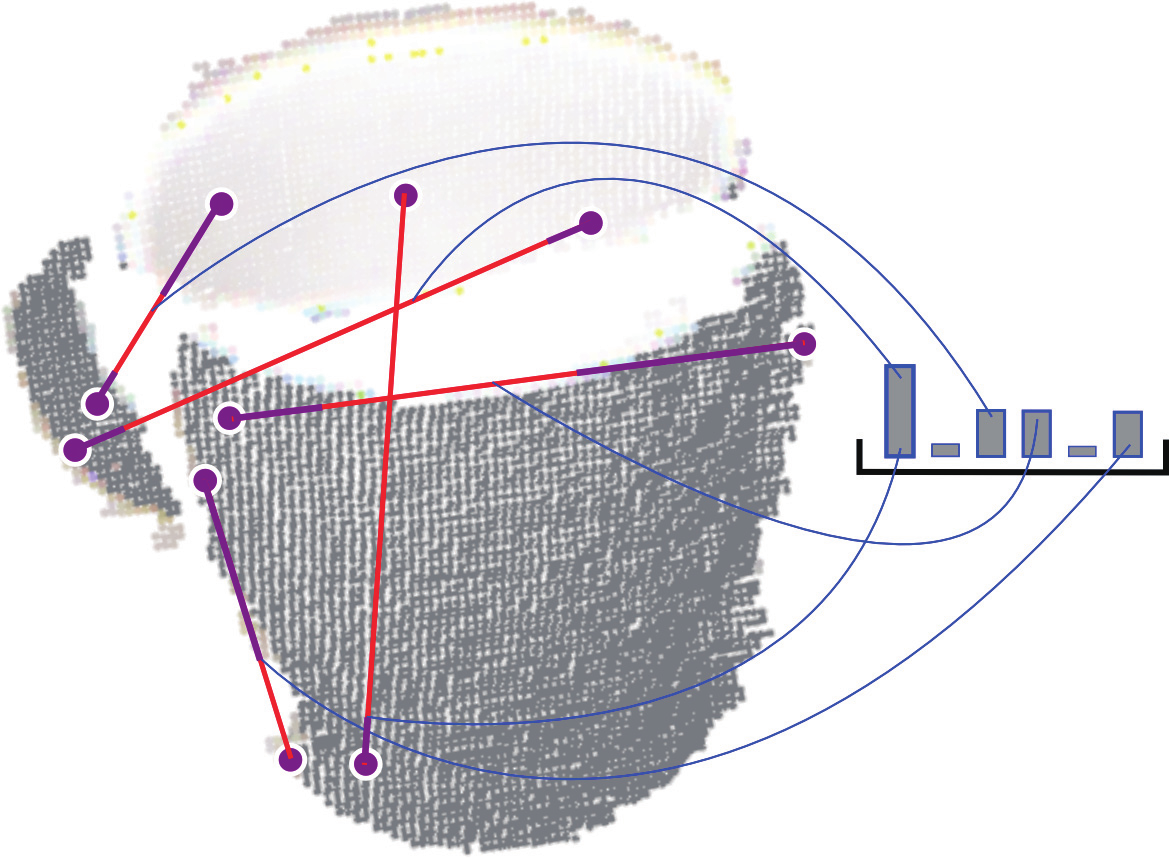
\includegraphics[width=0.23\textwidth]{images/wohl_ratio}
  }
  \subfloat[]{
    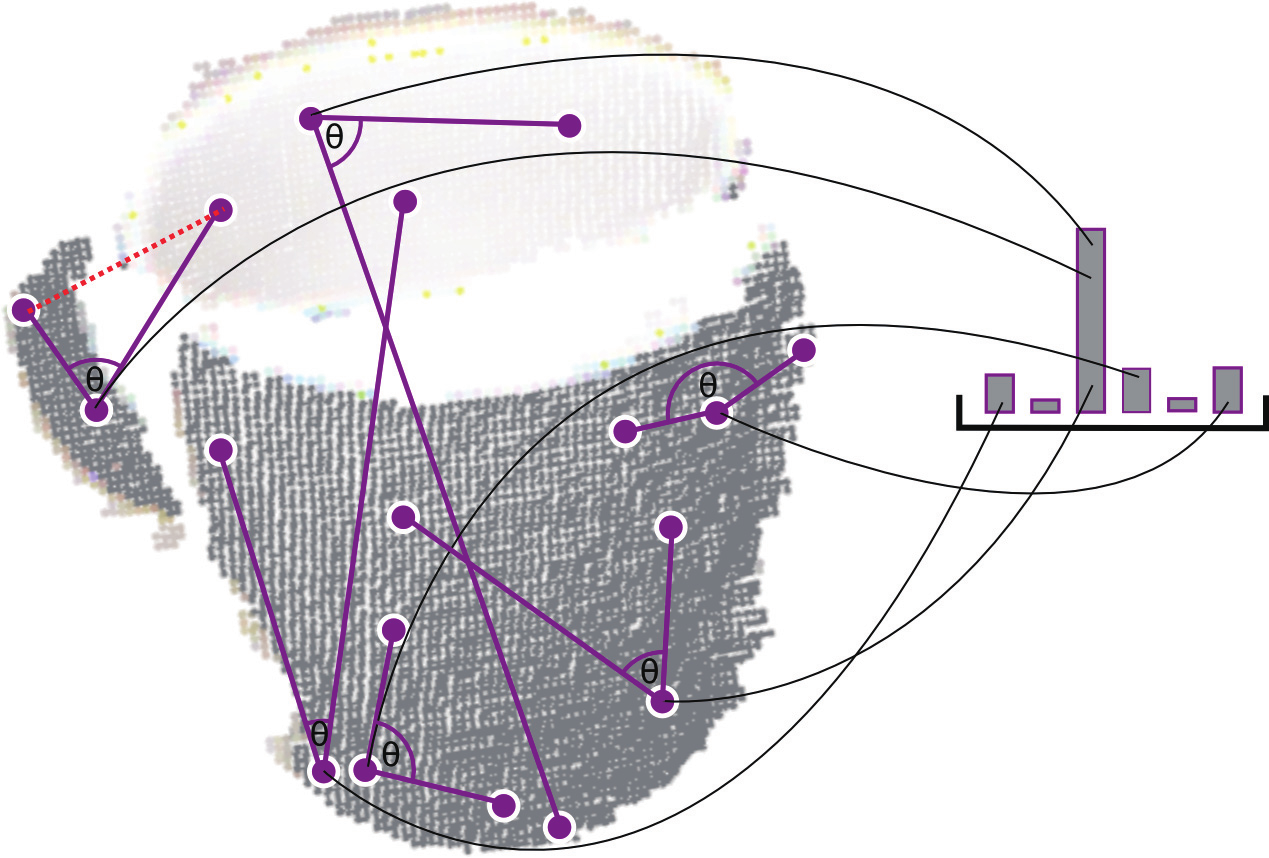
\includegraphics[width=0.23\textwidth]{images/wohl_a3}
  }
  \caption{Examples of the measures used to construct the Ensemble of Shape
    Functions histograms of \cite{wohlkinger2011ensemble}. a) Distance between
    points. b) Whether the points are on or off the model, or mixed. c) Ratio of
  line segments on and off the surface of the model. d) Angle between pairs of lines.}
  \label{fig:wohlESF}
\end{figure}

The splash descriptor was introduced by Stein et al. \cite{stein1992structural}.
A point on the surface with a given surface normal (the reference normal) is
chosen, and a slice around that with some geodesic radius (distance along the
surface) is computed. Points on the circle are selected using some angle step,
and the normal at that point is determined. A super splash is when this process
is repeated for several different radii. For each normal on the circle,
additional angles between it and a coordinate system centred on the reference
normal are computed. These angles and the angle around the circle are then
mapped into a 3D space, where polygonal approximation is made, connecting each
point with a straight line. Some additional computation is done to allow the
encoded polygons to act as a hash. Figure~\ref{fig:splash} shows part of the
formulation.

\begin{figure}
  \centering
  \subfloat[]{
    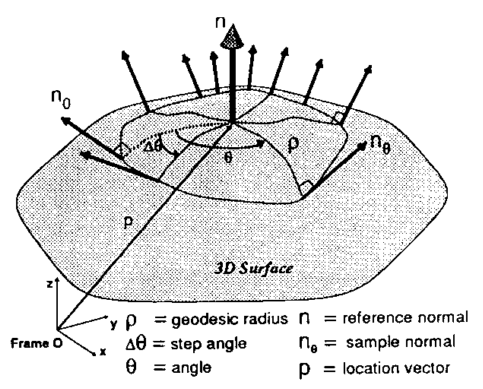
\includegraphics[width=0.32\textwidth]{images/splash}
  }
  \subfloat[]{
    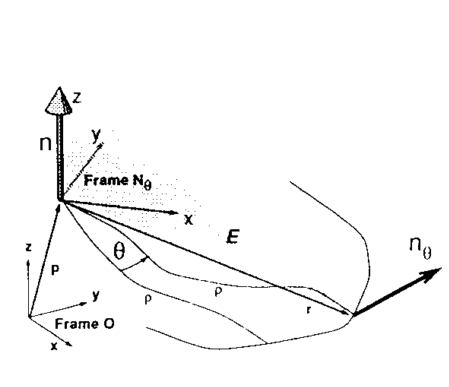
\includegraphics[width=0.32\textwidth]{images/splash_normals}
  }
  \subfloat[]{
    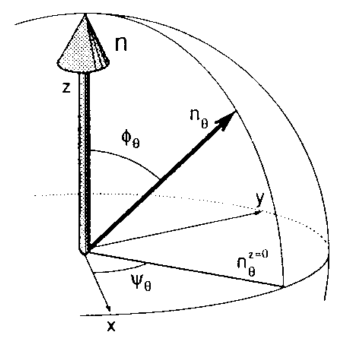
\includegraphics[width=0.32\textwidth]{images/splash_angles}
  }
  \caption{Splash descriptor \cite{stein1992structural}. a) shows the splash and
    normals around it. b) and c) show how the additional angles are defined.
  }
  \label{fig:splash}
\end{figure}

Point Signatures are similar to the splash descriptor in the sense that they
both sample points on a circle \cite{chua1997point}. This descriptor again
selects a reference normal, and has a specific radius. This time, the radius
defines a sphere around the point. The intersection of the surface with the
sphere is a 3D space curve. The orientation of the curve is defined by fitting a
plane to it. The distances between the space curve and the fitted plane at
sampled points define the signature of the reference point. These signatures can
be compared by lining them up and checking whether the query falls within the
tolerance band of previous signatures. Figure~\ref{fig:pointsig} shows
signatures from various surfaces.

\begin{figure}
  \centering
  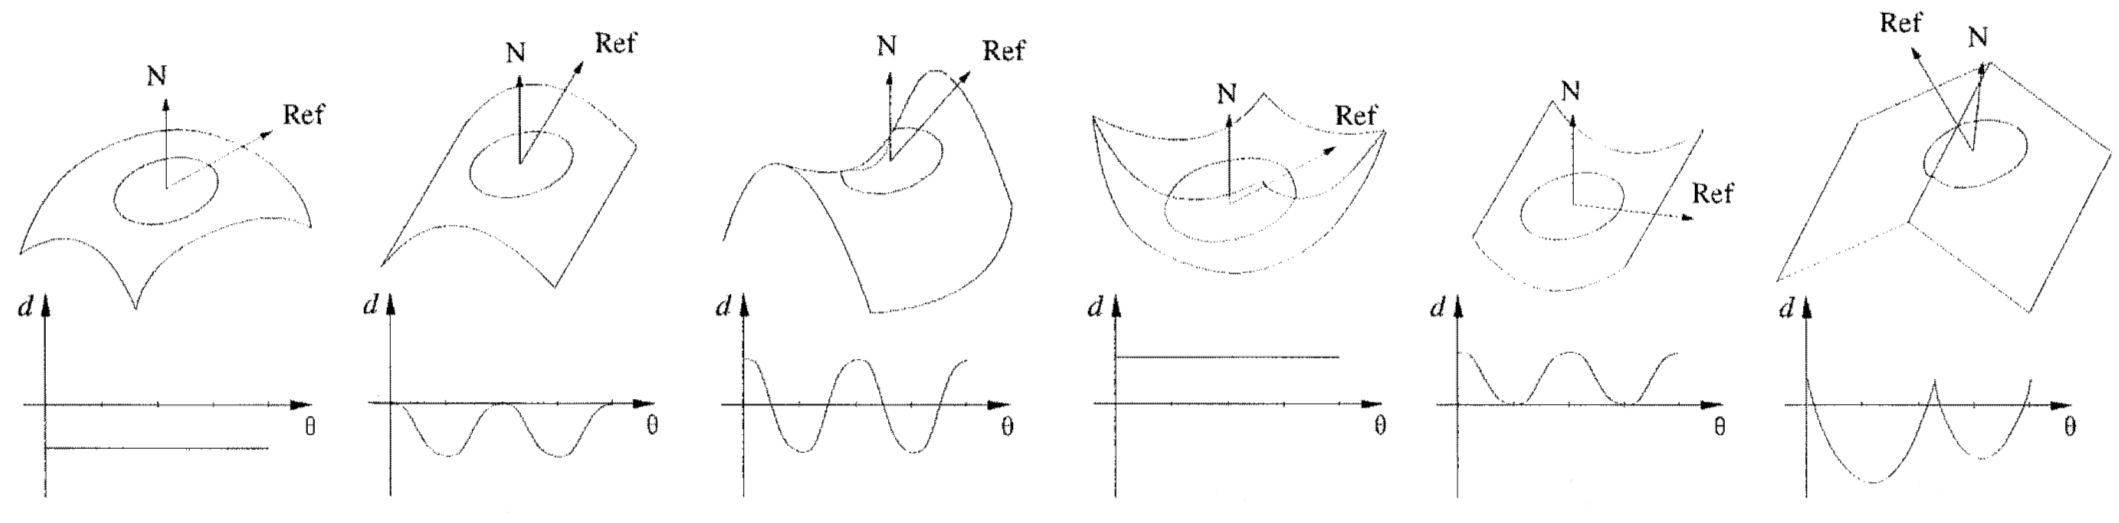
\includegraphics[width=\textwidth]{images/pointsig}
  \caption{Examples of the point signature responses to different surfaces
    \cite{chua1997point}. $d$ is the distance from the reference vector to the
    space curve defined by the intersection of the surface with a sphere centred
    at $N$. Ref rotates about $N$.}
  \label{fig:pointsig}
\end{figure}

\subsubsection{Descriptors With Interest Point Extraction}
While many descriptors designed for 2D applications also select interest points
during an initial step in the process, the 3D descriptors that we have mentioned
above do not automatically find locations in the cloud which are good points at
which to compute descriptors.

The Normal Aligned Radial Feature (NARF) is an interest point extraction method
with a feature descriptor. A score for the image points is determined based on
the surface changes at the point, and information about borders. An interest
value is computed from this based on the score of the surrounding points.
Smoothing is applied, and non-maximum suppression is applied to find the final
interest points. To compute the descriptor, rays are projected over the range
image from the centre at certain intervals. The intensities of cells lying under
the ray are weighted based on their distance from the centre, and a normalised
weighted average of the pairwise difference of cells is used to define each
element of the descriptor vector, which has a length equal to the number of rays
\cite{steder2011point}. The method is an improvement on a previous paper by the
authors \cite{steder2009robust}. A problem with this method is that it uses
range images directly. Point clouds can be used to generate range images by
looking at them from different viewpoints, but this adds complexity to the
method.

The integral volume descriptor is interesting as it combines interest point
selection and description into one. The descriptor is defined as the volume of
the intersection of a sphere centred at a point on the surface of an object with
the inside of the object (Figure~\ref{fig:volint}). Interest points are selected
by histogramming the descriptor values, identifying bins with a number of points
less than a specified values, and selecting points from these bins. To ensure
features are properly spaced, points in a certain radius of already selected
points cannot be used. By modifying the radius of the sphere used to generate
the descriptor, interest points at different scales can be selected
\cite{gelfand2005robust}.

\section{Matching Point Clouds}
\subsection{Point Matching}
In \cite{chui2003new}, Chui and Rangarajan introduce an extension to ICP which
allows for non-rigid registration and improved robustness to outliers. In
contrast to ICP, their approach does not use the nearest-neighbour approach to
define correspondence. Instead, they use an alternating algorithm similar to
expectation maximisation. Annealing is used to prevent binary correspondences
when the algorithm is not yet close to the solution --- at the beginning there
is a large search range for correspondences, which gradually shrinks as the
temperature decreases.

\subsection{Model Matching}
\begin{figure}
  \centering
  \subfloat[Conformal factors. High value indicates high required deformation to
  sphere \cite{ben2008characterizing}.]{
    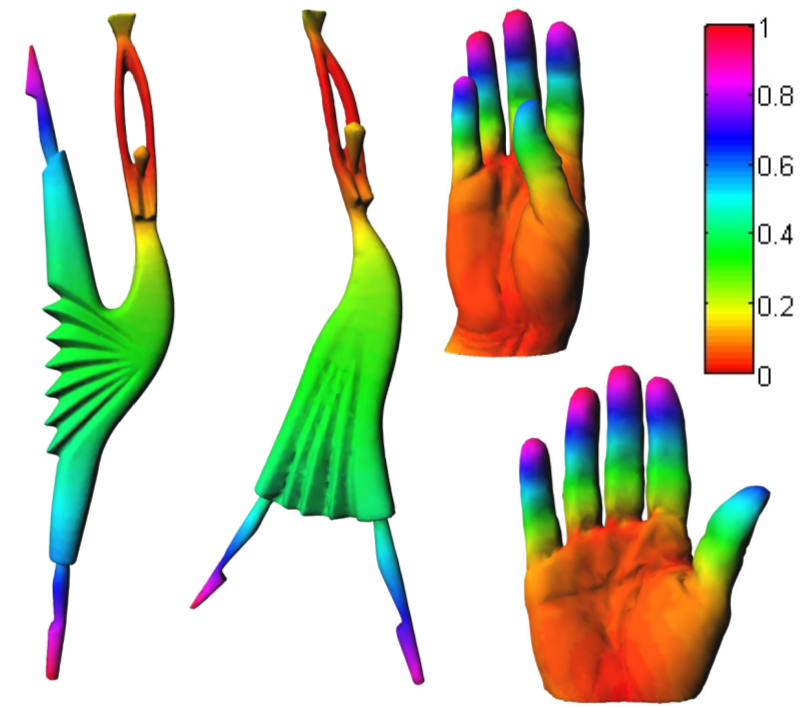
\includegraphics[width=0.48\textwidth]{images/conformal.png}
    \label{fig:conform}
  }
  \caption{Model matching approaches}
  \label{fig:modelmatch}
\end{figure}
In \cite{ben2008characterizing}, Chen et al. describe another approach to model
matching using conformal factors. This technique uses ideas from conformal
geometry, transforming the mesh of an object such that it has a uniform Gaussian
curvature. Information is stored about how much deformation is needed locally to
globally transform the object into a sphere --- this is the conformal factor.
The factor is based on a global computation on the whole mesh, as opposed to
per-vertex computations of the Gaussian curvature, which makes it much smoother
and appropriate for use in histograms. The histogram of a sample of the factors
is used as a descriptor, and is pose invariant, as seen in
Figure~\ref{fig:conform}. The authors say that it should be possible to use the
approach in partial model matching.

\section{Storing and Querying Descriptors}
There are several techniques for storing and querying descriptors, mostly based
on some form of tree. Recently, the k-d tree\cite{bentley1975multidimensional,
  friedman1977algorithm} has been used for efficient approximate matching with
either an error bound \cite{arya1998optimal}, where there is a bound placed on
the error between the true nearest neighbour and the one found, or a time bound
\cite{beis1997shape}, where the search is stopped after examining a certain
number of leaf nodes. Further improvements on the k-d tree are introduced in
\cite{silpa2008optimised}, where multiple randomised trees are used to optimise
the search. A priority search tree algorithm is introduced in
\cite{muja2014scalable}, which appears to be very effective. This may be the
same one as in \cite{muja2009fast}. The algorithm in the last two papers has
been integrated into PCL, which is useful.

A different approach to nearest neighbour search is the balltree, which uses
hyperspheres in a hierarchy to enclose points in the space
\cite{omohundro1989five}. Unlike the k-d tree, regions on the same level of the
tree are allowed to intersect, and do not need to partition the whole space,
which gives the balltree its representative power.

The vocabulary tree \cite{nister2006scalable} makes use of techniques from
document search to index images. Using $k$-means clustering, construction stage
creates a hierarchical quantisation of the image patch descriptors. In the query
phase, descriptors are compared to the cluster centres, and go down the tree
until a leaf is reached. The path through the tree is used as a scoring measure
to present retrieval results.

Philbin et al. \cite{philbin2007object} show that flat (single-level) $k$-means
clustering can be scaled to large vocabulary sizes if approximate nearest
neighbour methods are used. Early systems for image retrieval used a flat
clustering scheme, which could not scale to large vocabularies
\cite{sivic2003video}. The paper also introduces a re-ranking method which uses
spatial correspondences, which improves the retrieval quality.

Boiman et al. \cite{boiman2008defense} introduce the Naive Bayes Nearest
Neighbour (NBNN) classifier. It uses nearest neighbour distances in the space of
descriptors instead of images, computing ``image-to-class'' distances without
quantising the descriptors. In general, quantisation allows for dimensionality
reduction, at the expense of the discriminative power of descriptors. NBNN ``can
exploit the discriminative power of both (few) high and (many) low informative
descriptors''. The problem here is that the classes must be known beforehand,
and in our case we do not have that information. The local NBNN
\cite{mccann2012local} does not do the search based on classes. Instead, all the
descriptors are merged into a k-d tree on which approximate $k$-NN is run to
find descriptors in the local region of a query descriptor. A distance to
classes not present in the $k$-NN region is approximated by the distance to the
$k+1$th neighbour.

Funkhouser and Shilane present a method for querying a database of 3D objects
represented by local shape features \cite{funkhouser2006partial}. Partial
matches (correspondences) are stored in a priority queue sorted by geometric
deformation and the feature similarity. This means that only objects in the
database with a high probability of being a match need to be processed.

Some work has been done on optimising the retrieval of relevant images by
learning from user input \cite{rui2000optimizing}. When retrieved images are
presented, the user ranks them in terms of relevance, and this rank is then used
to improve the relevance of future searches.

\chapter{Preprocessing}
\label{chap:preprocess}
The first step in the object query system is to perform some preprocessing on
the clouds in the data set --- while not strictly necessary, there are some
benefits to doing so, chief of which is a reduction in computation time. The
data set that we have consists of around 80 clouds of a single room, taken at
different times during different days of approximately a month of time. The
clouds are made up of a number of intermediate frames, which are registered into
a complete cloud. The robot used to collect the clouds takes several sweeps of
the room, changing the angle of the camera after each sweep. The clouds are
constructed using frames taken from a sweep where the camera is pointing
slightly below the horizontal. Examples of the raw clouds can be seen in
Figure~\ref{fig:orig}.

We also have a number of subsets of the raw cloud which represent objects in the
raw cloud. These annotation clouds are generally quite small, varying in size
from 134 points to 14,149. We also apply some preprocessing steps for these
clouds.

\begin{figure}
  \centering
  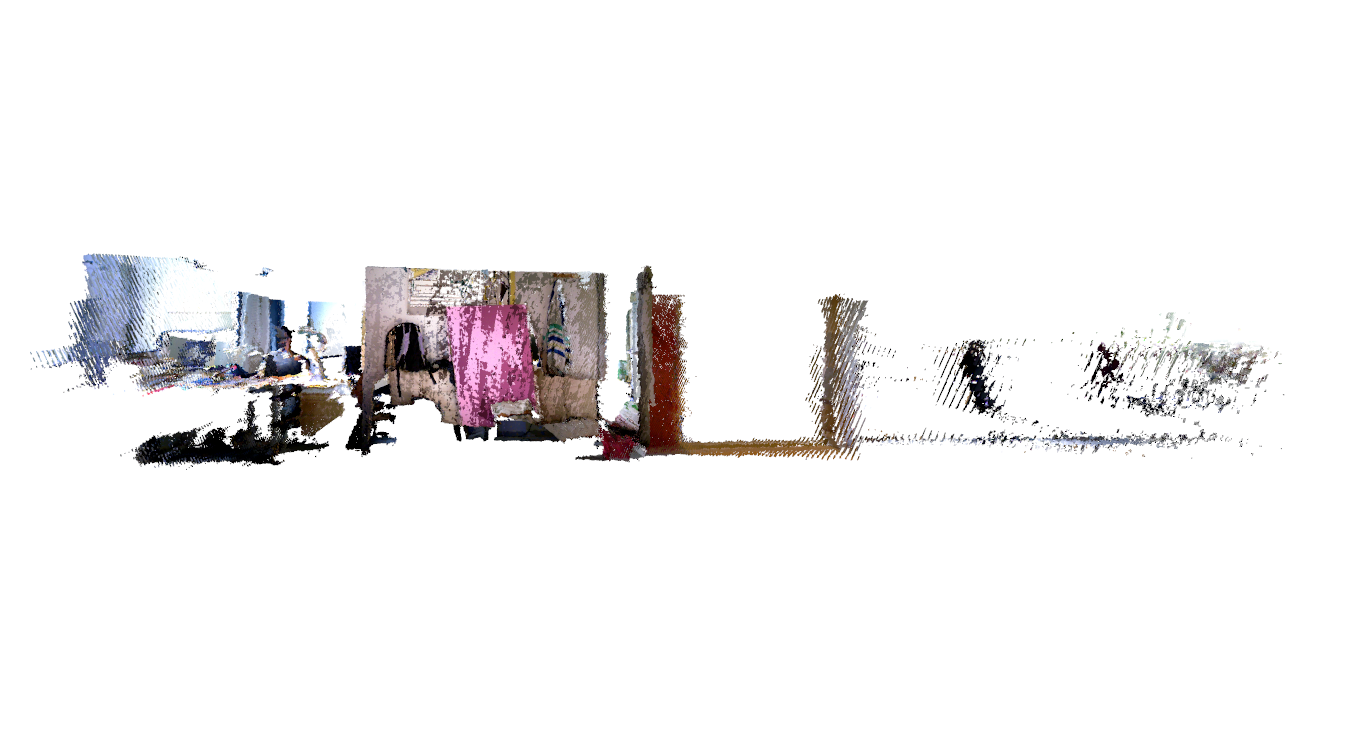
\includegraphics[width=0.49\textwidth]{images/orig_side}
  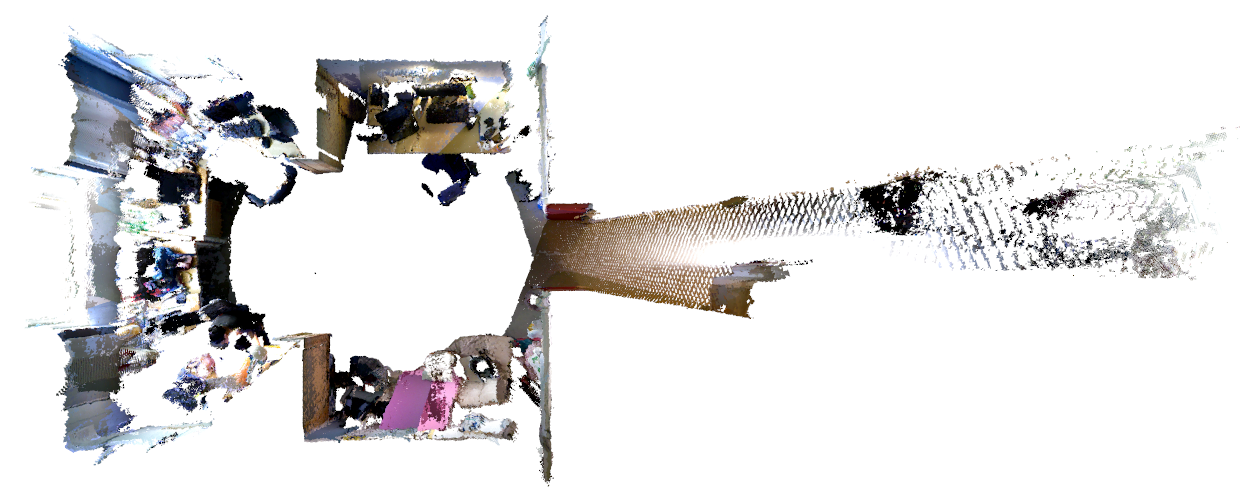
\includegraphics[width=0.49\textwidth]{images/orig_top}
  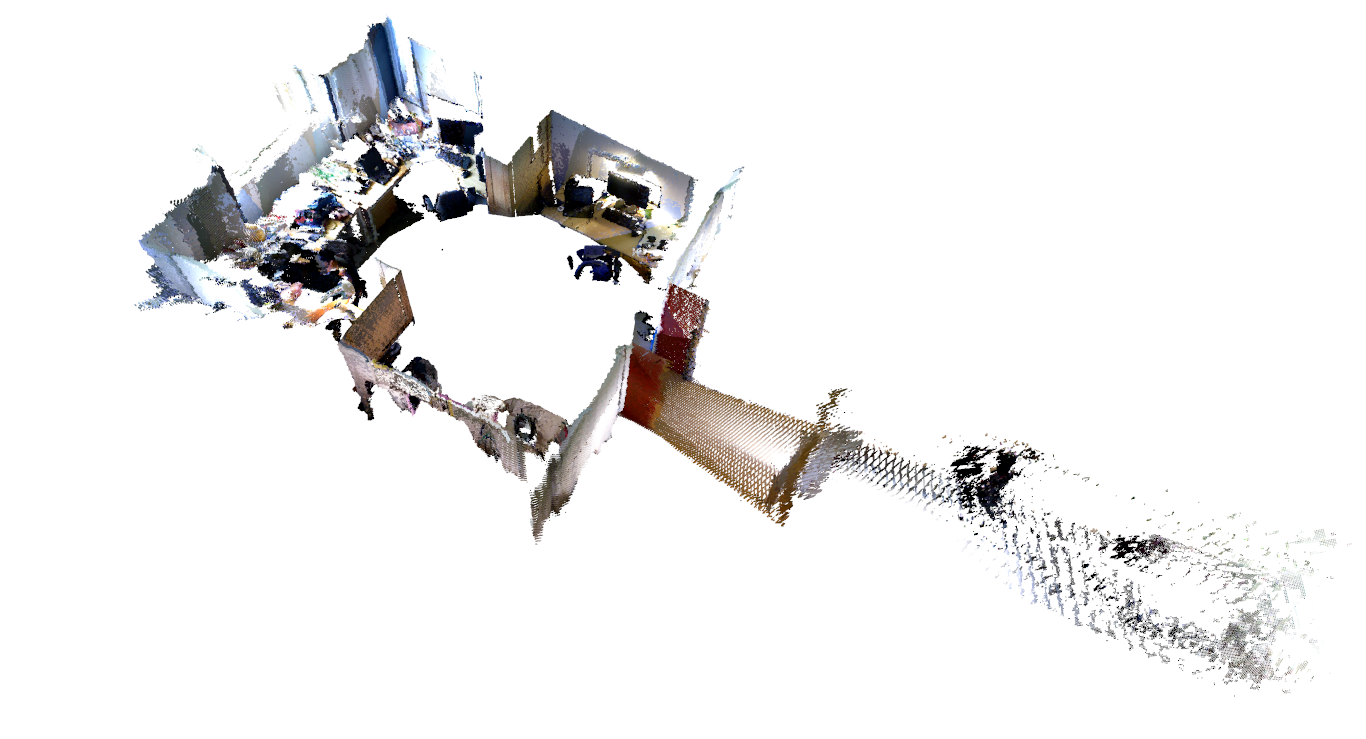
\includegraphics[width=0.49\textwidth]{images/orig_diag_left}
  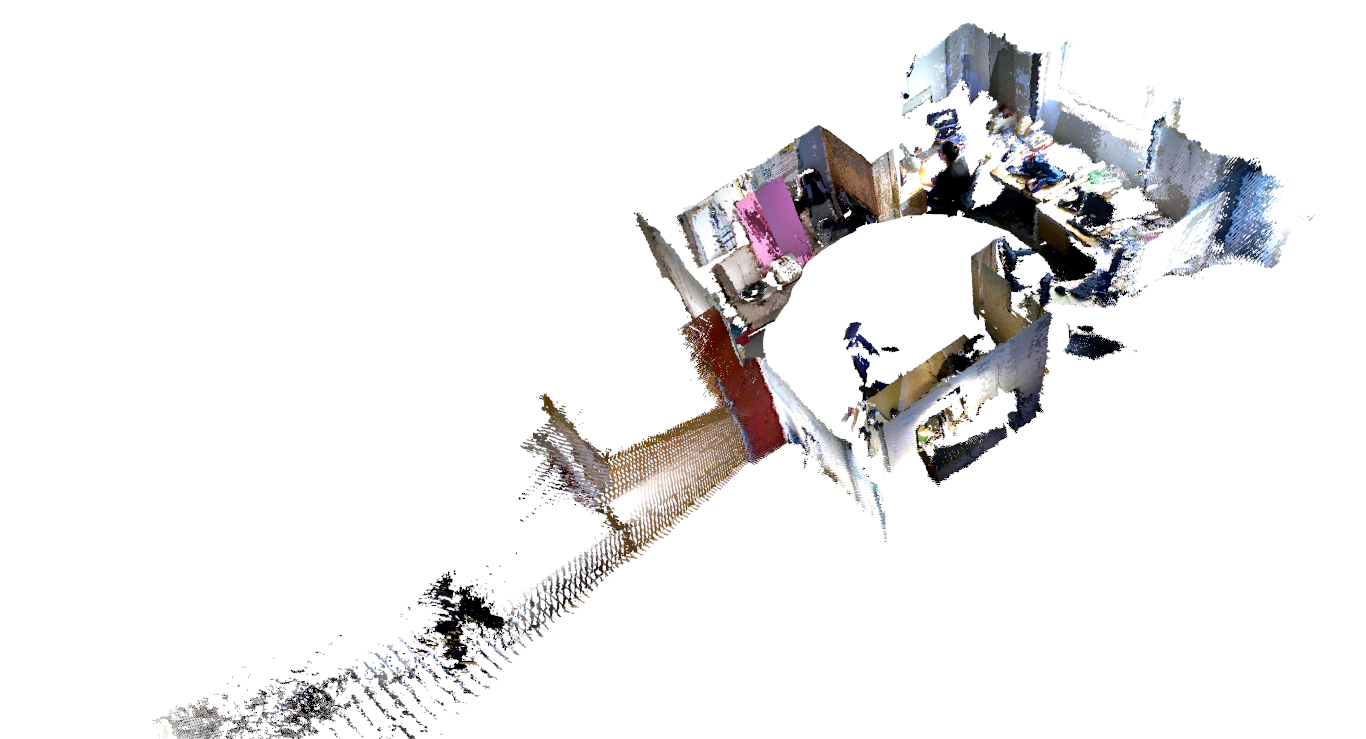
\includegraphics[width=0.49\textwidth]{images/orig_diag_right}
  \caption{Sample raw cloud viewed from several angles}
  \label{fig:orig}
\end{figure}

\begin{figure}
  \centering
  \subfloat[backpack1]{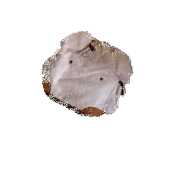
\includegraphics[width=0.30\textwidth]{images/annotations/original/backpack1_front_ut}}
  \subfloat[backpack2]{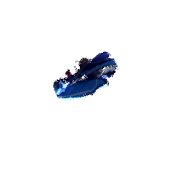
\includegraphics[width=0.30\textwidth]{images/annotations/original/backpack2_front_ut}}
  \subfloat[helmet]{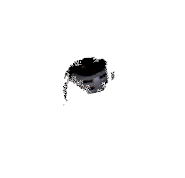
\includegraphics[width=0.30\textwidth]{images/annotations/original/helmet_front_ut}}\\
  \subfloat[chair3]{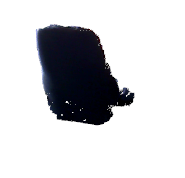
\includegraphics[width=0.30\textwidth]{images/annotations/original/chair3_front_ut}}
  \subfloat[pillow3]{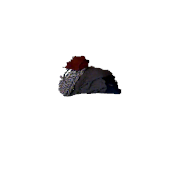
\includegraphics[width=0.30\textwidth]{images/annotations/original/pillow3_front_ut}}
  \subfloat[laptop1]{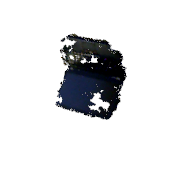
\includegraphics[width=0.30\textwidth]{images/annotations/original/laptop1_front_ut}}\\
  \subfloat[laptop2]{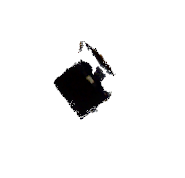
\includegraphics[width=0.30\textwidth]{images/annotations/original/laptop2_front_ut}}
  \subfloat[hanger\_jacket]{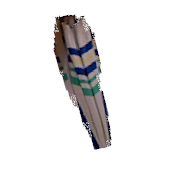
\includegraphics[width=0.30\textwidth]{images/annotations/original/hanger_jacket_front_ut}}
  \subfloat[trash\_bin]{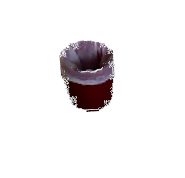
\includegraphics[width=0.30\textwidth]{images/annotations/original/trash_bin_front_ut}}\\
  \subfloat[chair1]{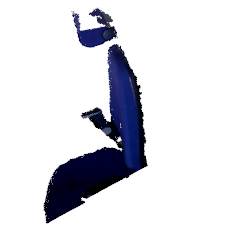
\includegraphics[width=0.30\textwidth]{images/annotations/original/chair1_front_ut}}
  \subfloat[chair2]{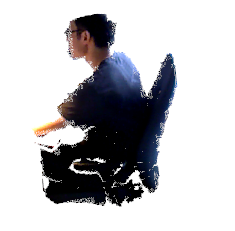
\includegraphics[width=0.30\textwidth]{images/annotations/original/chair2_front_ut}}
  \caption{Selection of objects from the dataset.}
  \label{fig:objects_ut}
\end{figure}

\section{Downsampling}
In their merged forms, the clouds on average contain approximately 4,300,000
points for a room which is around 4m wide, 5.5m deep and 3m high. This number of
points does not actually provide us with much additional information, since the
intermediate frames all have the same resolution. As such, we can safely
downsample the cloud to get a more reasonable number of points.

To downsample, we make use of a voxel grid, which splits the 3D space in which
the cloud sits into smaller subspaces of equal size called voxels. The width,
height and depth of voxels in the space can be specified, but we are interested
in keeping all dimensions the same resolution, and so we specify the parameters
so that each voxel is a cube. At this stage, we would like to perform a simple
downsampling to reduce the number of points, but we wish to keep small details
in the cloud --- something in the realm of a 1cm resolution is ideal in this
case.

Downsampling with a 1cm resolution gives a reduction in size of the clouds of on
average 78\%, to approximately 950,000 points.
Figure~\ref{fig:downsample_effect} shows the effect of the downsampling. While
there is slight degradation of the textures, this is to some extent a visual
effect which is viewpoint dependent. Most of the structure in the cloud is
retained, which is key. This step is important, as it greatly affects the speed
of computation of subsequent steps in the system, but it is a trade off. If the
downsampling resolution is too low, then we lose a lot of information about the
surface structure of parts of the cloud, and this is likely to lead to worse
performance when trying to find matches. How tolerant we are to low resolution
also depends on the kinds of objects that we are interested in finding. If we do
not care about smaller objects, then even with a lower resolution the results
should still be satisfactory. However, a lower resolution likely means that it
will be necessary to look at larger regions of space in order to describe
points. We will investigate the effects of this in chapter~\ref{chap:exp}.

Show some of the objects which are made up of slices due to viewing angle -
downsampling can reduce this slicing effect.

\begin{figure}
  \centering
  \centerline{
    \subfloat[Sofa]{
      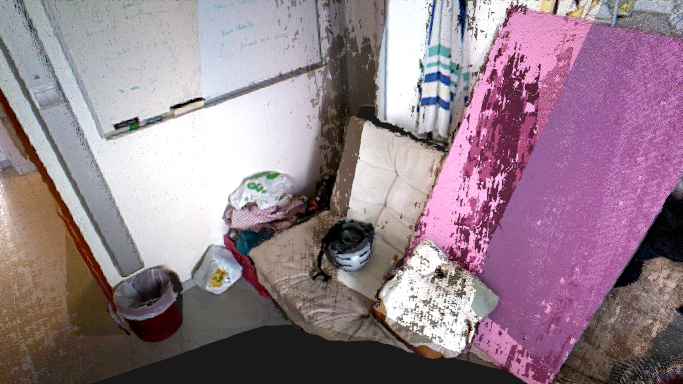
\includegraphics[width=0.60\textwidth]{images/sofa_og}
      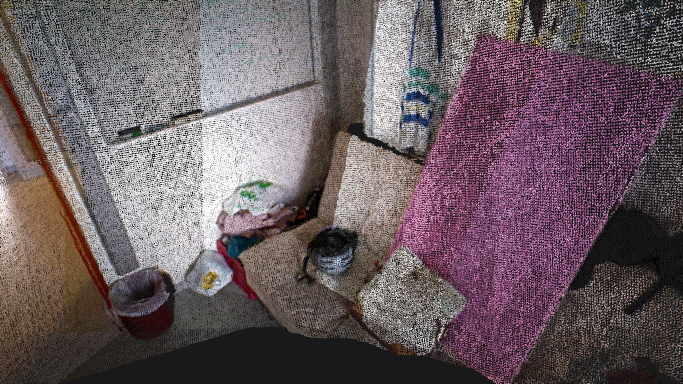
\includegraphics[width=0.60\textwidth]{images/sofa_ds}
    }\\
  }
  \centerline{
    \subfloat[Desk 1]{
      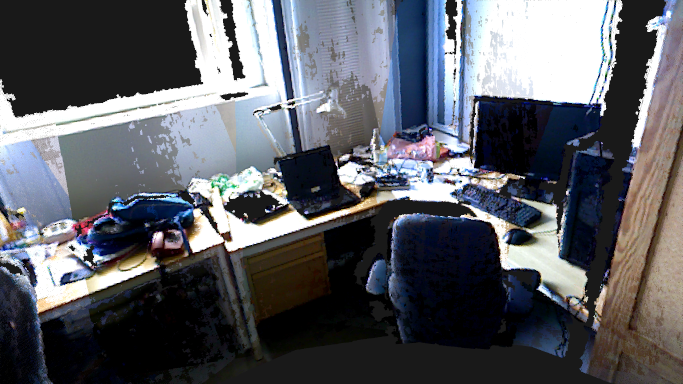
\includegraphics[width=0.60\textwidth]{images/johan_og}
      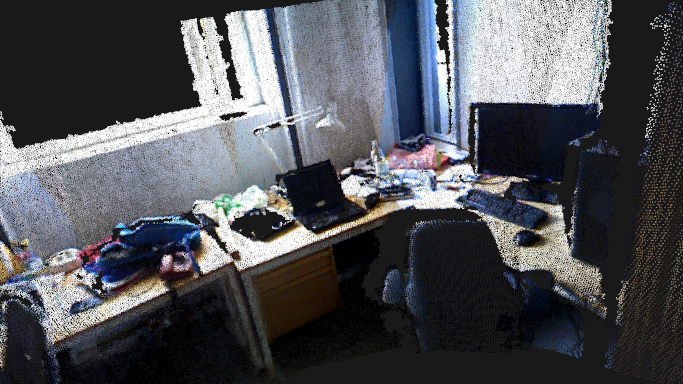
\includegraphics[width=0.60\textwidth]{images/johan_ds}
    }\\
  }
  \centerline{
    \subfloat[Desk 2 side]{
      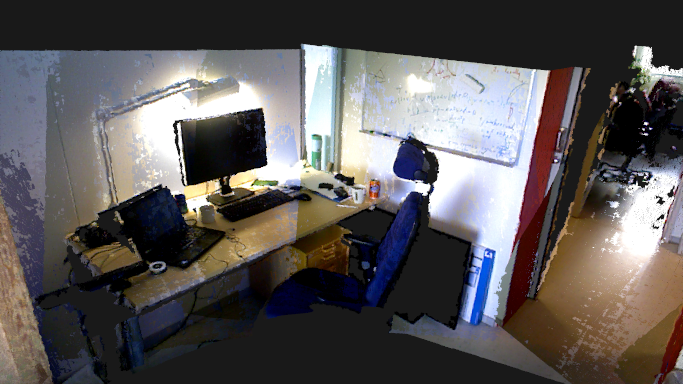
\includegraphics[width=0.60\textwidth]{images/nils_side_og}
      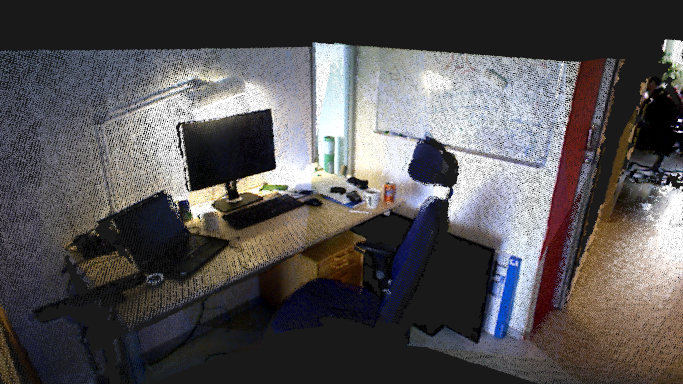
\includegraphics[width=0.60\textwidth]{images/nils_side_ds}
    }\\
  }
  \centerline{
    \subfloat[Desk 2 front]{
      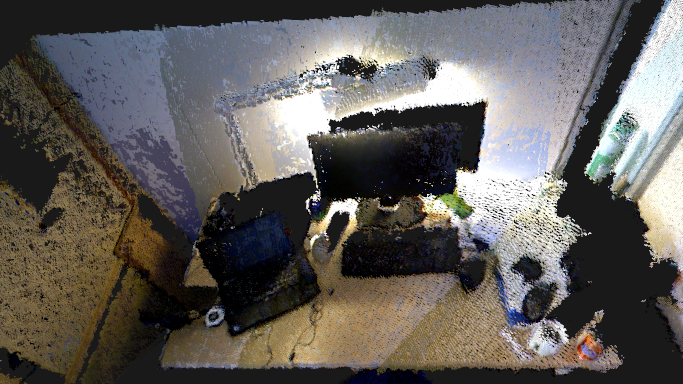
\includegraphics[width=0.60\textwidth]{images/nils_front_og}
      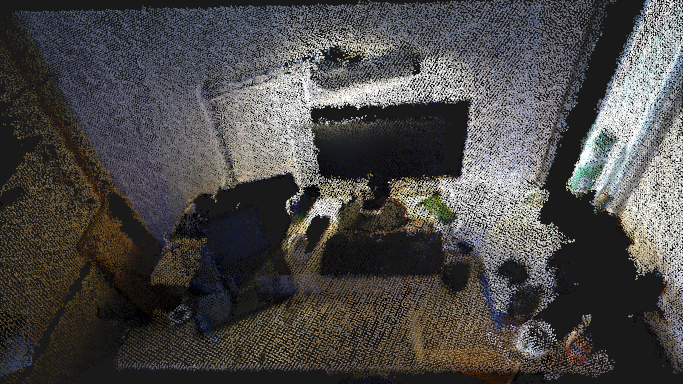
\includegraphics[width=0.60\textwidth]{images/nils_front_ds}
    }\\
  }
  \caption{The effect of downsampling. The left column shows the original
    clouds, the right column clouds downsampled with voxel size of 1cm$^3$.}
  \label{fig:downsample_effect}
\end{figure}

\section{Transformation and Trimming}
\begin{figure}[t]
  \centering
  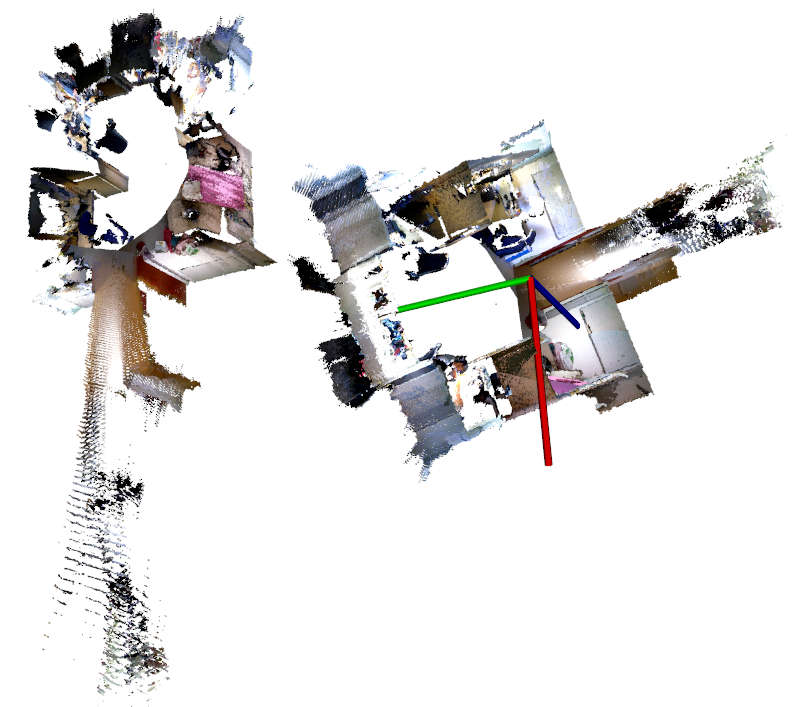
\includegraphics[width=0.8\textwidth]{images/orig_transformed}
  \caption{Original cloud and the transformed cloud. The original cloud
    is on the right. The coordinate axis shows the global reference frame ---
    none of the axes are aligned for the original cloud, but the transformed
    cloud is well aligned with the $x$-$y$ plane.}
  \label{fig:orig_transformed}
\end{figure}

Once the cloud has been downsampled, there is a little more that needs to be
done in order to get the cloud into a convenient form. The raw data that we have
has clouds which have their origin at the position of the camera while the room
was being scanned. Our data is a subset of a larger dataset which contains
clouds of more than one room --- if we were to use the data without applying any
additional transformations, all the clouds would sit on top of each other at the
origin, whereas we would ideally like to have them in their true position
relative to the origin. The robot collecting data knows its position, so this
information is stored.

As mentioned before, each cloud is a combination of a number of intermediate
frames, each of which has corresponding information about the pose of the camera
when the frame was taken, which we can use to transform the complete cloud into
its actual position in space.

An added benefit of this transformation is that it allows us to remove the floor
and ceiling by using a simple thresholding filter on the $z$ axis, as the floor
of the cloud is now aligned with the $x$-$y$ plane of the global reference
frame, as opposed to being aligned with the cloud's rotated reference frame
(Figure~\ref{fig:orig_transformed}) The threshold for the ceiling can be
determined by measuring the ceiling height, and the floor is assumed to be a
$z=0$. We add a small offset to each of the values to ensure that the parts are
correctly removed even if there is some noise.

Although we would like the system to be as generic as possible, the particular
subset of clouds that we are using have a large number of points outside the
room which do not give any useful information. To this end, we also include
additional filters on the $x$ axis to remove these points.
Figure~\ref{fig:trimmed} shows the end result of this step.

\begin{figure}
  \centering
  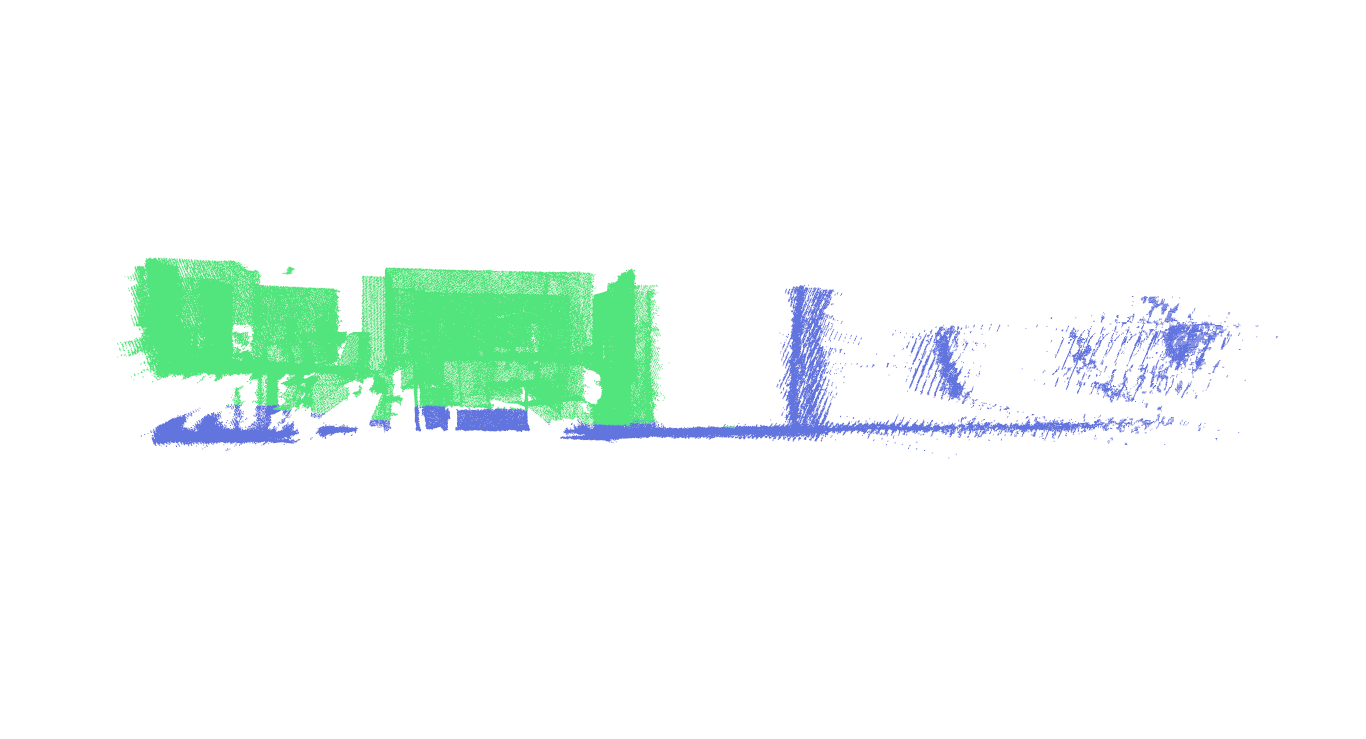
\includegraphics[width=0.45\textwidth]{images/trimmed_side}
  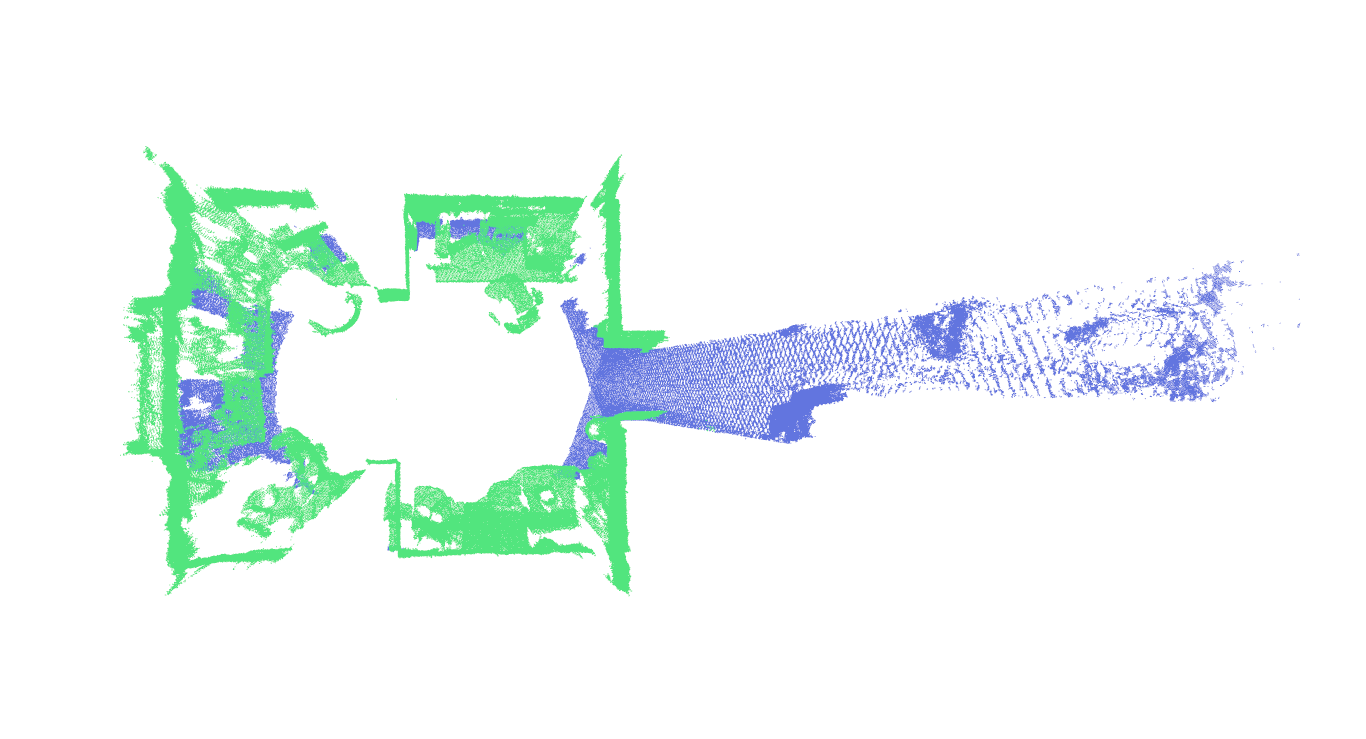
\includegraphics[width=0.45\textwidth]{images/trimmed_top}
  \includegraphics[width=0.45\textwidth]{images/trimmed_diag_left}
  \includegraphics[width=0.45\textwidth]{images/trimmed_diag_right}
  \caption{Result of trimming step. Transformed cloud is blue, trimmed is green.}
  \label{fig:trimmed}
\end{figure}

\section{Plane Extraction}
Having extracted normals from the cloud, we come to what is the most costly
preprocessing step. Due to the structured nature of our dataset, the number of
planes present in the clouds is quite high. While the presence of planes can be
used to define surfaces and the like, in our system we are not interested in
using the planes for anything in particular, and as such removing them from the
cloud is good, because we remove a large portion of points in the clouds which
are not be parts of any object, speeding up computation time of subsequent
steps. An example of the result of this step can be seen in
Figure~\ref{fig:plane_extr}.

\begin{figure}
  \centering
  
  \caption{Example of the result of plane extraction.}
  \label{fig:plane_extr}
\end{figure}

Plane extraction is done by running RANSAC multiple times with a plane model. A
plane can be described by its general form equation
\begin{equation}
  \label{eq:1}
  ax+by+cz+d=0
\end{equation}
where the normal vector $\mathbf{n}$ is defined by the coefficients $a$, $b$ and
$c$. To get the model coefficients, RANSAC samples three points ($p_1,p_2$ and
$p_3$) from the input cloud. From these three points, the normal is computed
using the cross product \cite{planeeq}

\begin{equation}
  \label{eq:2}
  \mathbf{n}=(p_2-p_1)\times(p_3-p_1)
\end{equation}

Once the plane coefficients have been computed, we must find the inlier points of this
plane model, based on their distance to the plane. The perpendicular distance of
a point $p$ to a plane is
\begin{equation}
  \label{eq:3}
  D=\frac{\mathbf{n}\cdot p + d}{\mid \mathbf{n} \mid}
\end{equation}

A point is considered to be an inlier if $D<D_t$, where $D_t$ is some threshold
on the distance. The RANSAC algorithm repeats the point sampling $n$ times,
storing the plane coefficients and number of inliers. At the end of the process,
the best plane the one with the largest number of inliers.

While this simple formulation can work well, there can be issues where the
planes that are extracted are not actually planes, due to there being regions in
the cloud where there can be a large number of inliers, but no actual plane, as
seen in Figure~\ref{fig:planenormal}. This effect can be mitigated by including
a single additional step to the inlier check, which also looks at the angle
between the plane normal and the normal at the point, computed by
\begin{equation}
  \label{eq:5}
  \theta=\cos^{-1}(\mathbf{n}\cdot p)
\end{equation}

A point is then considered an inlier only if it passes the distance threshold
check and $\theta<\theta_t$, where $\theta_t$ is the threshold on the angle.
This simple addition gives much more consistent results.

The RANSAC implementation that we are working with uses only a single distance
computation
\begin{align}
  \label{eq:6}
  D_a&=w\theta + (1-w)D\\
  w&=(1-p_c)w_n
\end{align}
where $p_c$ is the curvature at the point $p$, and $w_n$ is a predefined weight
on the distance between the point and plane normals. $p_c\rightarrow 0$ on flat
surfaces, so in these regions the normal will have a higher influence on the
aggregate distance $D_a$, whereas in regions of high curvature the euclidean
distance will be more important. Inliers are points where $D_a<T$.

\begin{figure}
  \centering
  
  \caption{RANSAC with basic plane model and with plane-normal model.}
  \label{fig:planenormal}
\end{figure}

When extracting planes, we use several parameters in addition to the aggregate
distance threshold $T$ to tweak the behaviour. The main aim of the additional
parameters is to prevent planes which are too small from being extracted. We
set a hard limit on the total number of planes which can be extracted, and also
define a threshold on the minimum number of points $N_{\min}$ in a plane.
\begin{equation}
  \label{eq:7}
  N_{\min}=\max(\eta N_{\text{trim}},\, N_{\text{fixed}})
\end{equation}
where $\eta$ is a small positive positive value. Since we are dealing with large
clouds, a suitable range of values is $\left[0.02,0.05\right]$.
$N_{\text{trim}}$ is the number of points in the trimmed cloud.
$N_{\text{fixed}}$ is a fixed value. We choose the maximum of the two values to
ensure that fluctuations in the cloud size are compensated for.

\section{Normal Estimation}
In this step, normals are estimated for each point in the cloud. The normal at a
point is the vector which is perpendicular to the curvature of the surface at
that point. By estimating normals for clouds, we can get some more information
about the surface structure of the cloud. Normals are used in several parts of
the system, including by feature selection methods and features. As mentioned
above, they are also used in the plane extraction step to increase accuracy.

There are many ways of estimating normals, but the method we use is formulated
as a least squares plane fitting problem, which is used to estimate the normal
of the plane tangent to the surface at the point at which the normal is to be
computed \cite{RusuDoctoralDissertation}. The computation gives an ambiguous
result in terms of the sign of the normal. To correct for this, a viewpoint is
needed, which serves to define what sign is used. Perhaps the most important
thing to note is that the normal must be computed using points in a
neighbourhood; either within a certain radius, or the nearest $k$ points. The
neighbourhood determines the scale factor that results. A small neighbourhood
gives a small scale factor, and a large neighbourhood a large scale factor. A
large scale factor can be bad if the objects that one is trying to examine have
regions where the rate of change of surface curvature is high, such as at the
corners of tables. It results in the smearing of edges and the suppression of
fine detail \cite{RusuDoctoralDissertation}. Figure~\ref{fig:normal_corner}
shows an example of the effect of different neighbourhood sizes on the results.

\begin{figure}
  \centering
  \includegraphics[width=0.49\textwidth]{images/normals_comb}
  \caption{Example of the smoothing effect of normal estimation radius. From
    bottom to top, 0.01, 0.025, 0.5, 0.2, 0.25, 0.5cm radius. Normals are
    indicated by orange lines. Note the tendency of normals with higher radius
    to tilt as they approach the corner. Normals on the top section are slightly
    skewed due to perspective.}
  \label{fig:normal_corner}
\end{figure}

Include figure with annotation objects with different normal radius

During preprocessing we compute two different sets of normals using different
settings for the radius. One set is for use with plane extraction, which has a
higher value for the radius, somewhat mitigating the effect of noise on the
normals, and resulting in less patchy extraction of planes
(Figure~\ref{fig:plane_normrad}).

\begin{figure}
  \centering
  
  \caption{Planes extracted with different settings for the normal radius}
  \label{fig:plane_normrad}
\end{figure}

\section{Annotations}
To ensure that the annotations for each cloud are in a similar form, we apply
the downsampling, transformation and normal extraction steps. The downsampling
step is particularly important here, as the raw annotations have issues with a
``slicing'' effect caused by the positioning of the camera when the frames were
taken, and its depth resolution (Figure~\ref{fig:slicing}). Using the raw clouds
to compute features would most likely result in worse performance as the surface
structure of the cloud is essentially a series of stacked planes, which would
lead to finding similar points anywhere where there is a flat surface.

\begin{figure}
  \centering
  \subfloat[Before downsampling]{
    \label{fig:slicing}
  }
  \subfloat[After downsampling]{}
  \caption{Annotations original and downsampled}
  \label{fig:annotation_ds}
\end{figure}
\chapter{Interest Point Selection}
\label{chap:interest}
Once the preprocessing step has been completed, we can move on to computing
features from the processed clouds. First, however, we need to choose the points
at which the descriptors will be computed. The idea of interest point selection
is to choose points in the cloud which are better in some way than other points
for feature extraction --- which points these are depends on the method used.
This is important, as if we can compute descriptors at locations which are
unique to an object, it makes any correspondences that are found when comparing
the descriptors likely to be actual occurrences of the object in the clouds in
which we are searching.

In this section we will describe in some detail the methods that we use. All of
the methods used are part of the PCL keypoints library \cite{pcl_keypoints}.

\section{Uniform}
The first and most obvious method of selecting points for feature extraction is
not to try to select interesting points at all, but to simply spread points
uniformly over the space. With this method, one would expect to extract a larger
number of points than with targeted methods, and since the entire space is
covered, it is unlikely that there will be any omissions of points that are
interesting.

The problem with having a large number of points is that this results in more
features having to be computed and compared in later stages.

To compute the uniform points, we simply downsample the cloud once more. The
size of the voxels used determines the spread of the points over the space ---
the behaviour of this method is determined entirely by a single parameter.
\section{ISS}
Zhong~\cite{zhong2009intrinsic} introduces the intrinsic shape signature
interest point selection method as one of a series of steps in the computation
of the ISS descriptor introduced in the same paper.

The main component of this method is the scatter matrix, which is the covariance
matrix of points within a spherical region around a sample point. For a point
$p_i$, the $3\times 3$ scatter matrix is
\begin{equation}
  \label{eq:4}
  S(p_i)=\sum_{\mid p_j - p_i \mid < r_s}(p_j-p_i)(p_j-p_i)^T
\end{equation}
where $p_j$ is another point in the cloud. $r_s$ defines the saliency radius,
which limits the points which we consider to be in the neighbourhood of $p_i$.
Interest points are only extracted in regions where there are at least $n_{min}$
points in the neighbourhood of $p_i$.

Once $S$ is computed, its eigenvalues $\lambda^1_i, \lambda^2_i$ and
$\lambda^3_i$ (with decreasing magnitude) are extracted. The smallest eigenvalue
$\lambda^3_i$ can be used to measure the 3D point variations in the
neighbourhood of the point \cite{zhong2009intrinsic}. If it happens that two of
the eigenvalues computed are equal, the reference frame of the point can become
ambiguous, so limits are applied to the ratio of the eigenvalues such that
\begin{equation}
  \label{eq:8}
  \frac{\lambda^2_i}{\lambda^1_i}< \gamma_{21},\, \frac{\lambda^3_i}{\lambda^2_i}< \gamma_{32}
\end{equation}

With this formulation, it is likely that more points are considered interest
points than are not. To thin the interest points further, non-maximum
suppression is used. Essentially, this removes from the interest points any
point where the value of $\lambda^3_i$ at the point is not the maximum in the
neighbourhood of the point. This neighbourhood is defined by the radius $r_{n}$,
whose value is usually distinct from the value of $r_s$.
\section{SUSAN}
The SUSAN (Smallest Univalue Segment Assimilating Nucleus) detector is based on
an algorithm introduced for 2D feature detection by Smith~\cite{smith1997susan}.
We use an extension of this detector to 3D. The basis for the SUSAN principle
comes from the concept of each image point having an associated local area which
has intensity and normal direction values that are similar to it.

A spherical region called the mask is defined, with some radius $r_m$ which has
at its centre a point referred to as the nucleus. Looking at the points within
the spherical region, we compare their values of the normal direction and
intensity to the nucleus values. From this comparison, a region of space which
has similar values to the nucleus can be defined. This region is known as the
univalue segment assimilating nucleus or USAN. Figure~\ref{fig:susan_nucleus}
shows this principle in the 2D case. The USAN contains information about the
structure of the cloud in small region. Depending on the position of the nucleus
in the cloud, the volume of the USAN will vary. In regions where all points are
similar, the USAN is large, and it is small when the region has a large
variation in point intensity and normal direction. Based on this observation,
using the inverted USAN volume as a feature detector should result in the
selection of descriptive points --- hence the name \emph{Smallest} USAN.

\begin{figure}
  \centering
  \includegraphics[width=0.48\textwidth]{images/susan1}
  \includegraphics[width=0.48\textwidth]{images/susan}
  \caption{Concept of nucleus and mask in 2D SUSAN detector. USAN is the white
    region in the right image \cite{zhang2013susan}.}
  \label{fig:susan_nucleus}
\end{figure}

To compute SUSAN keypoints, the following process is applied to each point $p_i$
in the cloud. First, all points $p_j$ in the neighbourhood defined by $r_m$ are
found. We then define the USAN and the centroid of the mask. In order to be
considered as part of the USAN, a point must fulfill the inequalities
\begin{align}
  \label{eq:9}
  \left|I_i-I_j\right|&\leq I_t\\
  1-\mathbf{n}_i\cdot\mathbf{n}_j&\leq \theta_t
\end{align}
where $I$ is the intensity of a point, and $\mathbf{n}$ is the normal, and $I_t$
and $\theta_t$ are user-defined thresholds on the intensity and angular
difference. The intensity is computed from RGB values using
\begin{equation}
  \label{eq:10}
  I=\frac{r+g+b}{3}
\end{equation}

We assume that each channel of the RGB value of a point has the same weight.

The centroid $C$ is computed using
\begin{equation}
  \label{eq:11}
  C=\frac{1}{\left|\text{USAN}\right|}\sum_{p_j \in \text{USAN}}p_j
\end{equation}

The last thing to do for each point is to ensure that the number of points in
the USAN is within the bound
\begin{equation}
  \label{eq:13}
  0 < \left| USAN \right| < 0.5(N-1)
\end{equation}
where $N$ is the number of points in the neighbourhood of the nucleus. If this
check is successful, the output intensity of the nucleus is set to
$I_o=0.5(N-1)-\left|USAN\right|$. This defines the response of the feature
selection at this nucleus.

% Some additional validation can also be applied to the
% point, checking that the distance $\mid\mid p_i-C\mid\mid<d_t$, where $d_t$ is a
% user-defined threshold on the distance. 
% If either the geometric threshold check or nucleus check fail, the point is
% not included in the interest point set.

Once $I_o$ has been computed for all valid points in the cloud, non-maximum
suppression is applied. Only those points which have the minimal intensity in
the neighbourhood defined by $r_m$ are used as the final interest points.

\section{SIFT}
The scale invariant feature transform, introduced by
Lowe~\cite{lowe2004distinctive} in 1999, it is still commonly used for many 2D
image processing applications. The most important concept introduced in the
paper is that of scale invariance --- the SIFT feature extraction method
automatically selects features at different scales. This effect is achieved by
applying a Gaussian blur with different standard deviation in 2D, and by
downsampling clouds in 3D. The leaf size used for downsampling is determined by
the number of \emph{octaves} $N_o$. Within each octave, there are several
\emph{scales} $N_s$ which are applied. After all scales in an octave have been
computed, the leaf size is doubled, and the process repeated, until it has been
applied to all octaves.

For each octave, the procedure begins with downsampling the point cloud to the
scale defined for that octave $S_{o}$, which initially is set to the minimum
scale $S_{\min}$. The scales in the octave are then defined by
\begin{equation}
  \label{eq:14}
  s_i=\frac{S_o\cdot 2^{i - 1}}{N_s}
\end{equation}
where $0<i<N_s$. Each point $p$ in the cloud has its nearest neighbours $P_{nn}$ computed,
within a radius three times the maximum scale $s_{N_s}$ in that octave. The same
neighbours are used for computation of the difference of Gaussians $D$ for each
scale in the octave. In each scale, a Gaussian response $R$ is computed
\begin{equation}
  \label{eq:15}
  R_i=\frac{\sum_{q\in P_{nn}}0.299q_r + 0.587q_g +
    0.114q_b\exp\left\{-\frac{0.5}{\sigma}\mid\mid p-q\mid\mid\right\}}{\sum_{q\in P_{nn}}\exp\left\{-\frac{0.5}{\sigma}\mid\mid p-q\mid\mid\right\}}\\
\end{equation}
$q_r$, $q_g$ and $q_b$ are the red, blue and green channels of the colour at the
point $q$, $\sigma=s_i^2$. The difference of Gaussians is then
\begin{equation}
  \label{eq:16}
  \text{DoG}_i=R_i-R_{i-1}
\end{equation}
where $1<i<N_s$. These values are then used to find extrema in the scale space.
The neighbourhood of each point is examined again, and the maximum and minimum
values of the DoG at any point within the neighbourhood are found for each
scale. For consideration as an interest point, the value of DoG$_i$ must be
greater than a minimum contrast threshold $t_c$. This limits the inclusion of
points where the responses are not very different. If this threshold is
exceeded, the value of DoG at the point is checked to see if it is a maximum or
a minimum in its neighbourhood, and is either larger or smaller than the maximum
and minimum values for the same point in the neighbouring scale spaces. If all
these criteria are fulfilled, the point is added to the interest points.

Once this process is completed for a single octave, the scale $S_o$ is doubled,
and the process repeats $N_o$ times. The selected interest points are the
aggregated results from each individual octave. 

\section{Harris}
Like SIFT, the Harris detector, introduced by the eponymous
Harris~\cite{harris1988combined}, was originally used as a method for edge and
corner detection in images. Much like ISS, it uses a covariance matrix applied
to the neighbourhood of a point as the basis of its function. Rather than using
the points themselves, however, the Harris detector finds the covariance matrix
of the normals in the neighbourhood. The response at the point is then computed
by combining the determinant and trace of the matrix. The resulting responses
for each point are then thinned using non-maximum suppression, and the remaining
points are the interest points.
\chapter{Descriptor Extraction}
\label{chap:descriptors}
In this step, we compute descriptors at each of the locations that was selected
by the interest point method that was used. The end goal of the combination of
the interest point selection and descriptor extraction steps is to produce a set
of descriptors that can be used to represent the scene without having to keep
all of the original data. In addition, putting information about the scene into
a compact representation also allows the comparison of two scenes much more
quickly than would otherwise be possible. Instead of comparing complex
structures in the scene, simple vectorial representations are compared instead.
The intention is to compute these representations and have them stored, so that
they can be accessed later to compare to the descriptors extracted from query
objects. Correspondences between descriptors from the query object and parts of
the room clouds should indicate the presence of the object in that cloud. We
will try to use this to more reliably retrieve objects.

However, finding a compact representation that is also distinctive enough and
produces similar results for similar regions of space is not easy. In the image
processing literature, a lot of work has been done to develop novel descriptors
which are faster to compute, are invariant to more effects that might reduce
their effectiveness, and better represent the image data. As with interest point
selection methods, current methods in 3D often make use of the lessons learned
from the development of 2D methods. 

\section{SHOT}
\begin{figure}
  \centering
  \includegraphics[width=\textwidth]{images/shotcolor}
  \caption{Representation of the construction of the SHOTCOLOR descriptor and
    the subdivisions used for local histogram computation.}
  \label{fig:shotcolor}
\end{figure}
The signature of histograms of orientations descriptor is the product of a study
on 2D descriptors, particularly SIFT, and makes extensive use of histograms, as
the authors believe that this is part of the reason why the descriptor is so
effective \cite{tombari2010unique}. The paper also discusses the importance of
the local reference frame, or RF. Defining a local RF is a way to ensure that
the same descriptor will be computed if the same points are translated or
rotated, or if there is noise or clutter in the region the descriptor algorithm
uses to define the descriptor values. This is analogous to the problem of
rotation and scale invariance in 2D descriptors. The RF is computed based on the
eigenvalue decomposition of a special scatter matrix $M$
\begin{equation}
  \label{eq:12}
  M=\frac{1}{\sum_{i:d_i\leq R}(R-d_i)}\sum_{i:d_i\leq R}(R-d_i)(\mathbf{p}_i-\mathbf{p})(\mathbf{p}_i-\mathbf{p})^T
\end{equation}
where $R$ is the radius used to define the neighbourhood used to compute the
descriptor, $\mathbf{p}$ is the point at which the feature is to be computed,
$\mathbf{p}_i$ is another point in the cloud, and $d_i$ is the euclidean
distance between $\mathbf{p}_i$ and $\mathbf{p}$.

The addition made by the authors to previous work is to use a weighted linear
combination, where the weight of a point is lower the further it is from the
central point. This is in order to reduce the effect of clutter. The eigenvalue
decomposition alone is not sufficient to define an unambiguous RF. To do so, the
authors use a technique introduced in \cite{bro2008resolving}, which orients the
signs of the eigenvectors to make them coherent with those of the points that
they are representing.

Having defined the local RF, information about the location of points within $R$
is accumulated to create the descriptor. This is done by computing local
histograms within subdivisions of the spherical region, and then grouping them
together to form the final descriptor. The spherical region is split into 32
regions by splitting the sphere along the radial, azimuth and elevation axes, as
seen in Figure~\ref{fig:shotcolor}. Points in each subdivision are grouped into
bins of the local histogram according to the cosine of the angle between their
normals and the normal of the feature point $\mathbf{p}$. This formulation
reduces computation time, and does not require complicated binning. Using the
actual angle to allocate points to bins has the disadvantage of needing
different bin resolutions depending on whether directions are close to or
orthogonal to the normal direction \cite{tombari2010unique}.

\section{SHOTCOLOR}
In a subsequent paper, the authors of SHOT introduce an extension to the
descriptor which also includes colour information \cite{tombari2011combined}. To
include colour information, the same histogramming method is applied, but
instead of using the dot product of the RGB vectors at the feature point and a
neighbourhood point, the authors use the $L_1$ norm of the RGB value converted
to the CIELab colour space. The value a pair of points is therefore
\begin{equation}
  \label{eq:17}
  l(C_p, C_q)=\sum^3_{i=1}\mid C_p(i)-C_q(i)\mid
\end{equation}
where $C$ is the CIELab colour triple of a point.

\section{USC}
Another descriptor introduced by Tombari is the universal shape context
\cite{tombari2010uniquesc}. This descriptor is an improvement of the 3D shape
context, in the sense that it has a unique reference frame, constructed in the
same way as for SHOT. As with SHOT, a spherical region is defined by a radius
$R_s$ and a central point, and separated into a number of bins. For each point,
the number of points $N$ in a local region defined by radius $R_d$ is computed.
A weighting $w$ for this point is then computed according to
\begin{equation}
  \label{eq:18}
  w=\frac{1}{N}V_b
\end{equation}
where $V_b$ is the volume of the bin that the point falls within. For each
point, $w$ is accumulated in the descriptor vector according to the bin into
which it falls. The final descriptor is therefore a representation of the
combined weights of all of the points in the sphere.
\section{PFH}
\begin{figure}
  \centering
  \includegraphics[width=0.48\textwidth]{images/darboux}
  \caption{Darboux frame defined by the vectors $u$, $v$ and $w$ \cite{rusu2008learning}.}
  \label{fig:darboux}
\end{figure}
The point feature histogram is the first in a family of descriptors described by
Rusu et al. \cite{rusu2008aligning}. The descriptor was developed in order to
improve performance of cloud matching with iterative closest point (ICP). Most
of the descriptors used for that purpose previously had only a single dimension,
and as a result could not be properly descriptive over a whole scene. The
descriptor is likely to have a similar value at different points in the scene,
which causes problem as one cannot have a high confidence that a correspondence
between two points in two different scenes is the correct one.

To solve this problem, the PFH descriptor uses 16 dimensions, computed based on
histograms, which allow for more distinctive features. As with all other
descriptors, operations are done on points within a radius $r$ of the central
point $p$. Each pair of points in the neighbourhood is examined, as in
Figure~\ref{fig:pfhinfluence}. In each pair, a source point $p_s$ and a target
point $p_t$ are determined by looking at the normals of the points, and
comparing the angles relative to the line connecting the two points. The point
whose normal has the smaller angle is the source, the other the target. A
reference frame with the origin as the source point is defined using the normal
of the source $n_s$ as
\begin{align}
  \label{eq:19}
  u&=n_s\\
  v&=(p_t-p_s)\times u\\
  w&=u\times v
\end{align}
as shown in Figure~\ref{fig:darboux}.

Using this frame, four features are computed
\begin{align}
  \label{eq:20}
  f_0&=v\cdot n_t\\
  f_1&=\mid\mid p_t - p_s\mid\mid\\
  f_2&=\frac{u\cdot(p_t-p_s)}{f_1}\\
  f_3&=atan(w\cdot n_t,u\cdot n_t)
\end{align}
where $n_t$ is the normal of the target point. These values are then used to
compute an index
\begin{equation}
  \label{eq:21}
  idx=\sum^3_{i=0}\left\lfloor \frac{f_i\cdot d}{f_{i\max}-f_{i\min}}\right\rfloor\cdot d^i
\end{equation}
that defines which of the histogram bins the pair of points falls. $d$ is the
number of divisions to apply to the possible feature value range
$f_{i\max}-f_{i\min}$.

Because this descriptor computation operates on \emph{all} point pairs in the
neighbourhood, depending on the size of the neighbourhood and the point density,
computation can be slow.
\begin{figure}
  \centering
  \subfloat[PFH]{\includegraphics[width=0.48\textwidth]{images/pfh}}
  \subfloat[FPFH]{\includegraphics[width=0.48\textwidth]{images/fpfh}}
  \caption{Influence diagrams of the PFH and FPFH descriptors \cite{rusu2009fast}.}
  \label{fig:pfhinfluence}
\end{figure}
\section{FPFH}
The fast point feature histogram was introduced to tailor the PFH descriptor to
real time applications while maintaining its discriminative power
\cite{rusu2009fast}. Instead of computing the values in Equation~\eqref{eq:19}
for every pair of points in the neighbourhood of $r$, they are only computed for
each point and its $k$ neighbours $p_k$ within the same radius --- this is
called the simplified point feature histogram (SPFH). Because of the use of two
neighbourhoods, the final descriptor can include information from points up to
$2r$ away. Once the SPFH value for each point in the neighbourhood is computed,
it is integrated into the final FPFH descriptor using
\begin{equation}
  \label{eq:20}
  FPFH(p)=SPFH(p)+\frac{1}{k}\sum^k_{i=1}\frac{1}{\omega_k}\cdot SPFH(p_k)
\end{equation}
where $k$ is the number of neighbours within $r$ and $\omega_k$ is the distance
between $p$ and $p_k$.

Because only direct neighbours of each point are considered, some
interconnections that would exist in the PFH computation do not in FPFH, which
contributes to its increased speed. The downside of this is that some of the
geometric structures which exist in the region will not be included. In
addition, due to the nature of the computation, the values for some points will
be factored into the descriptor twice.

A further improvement made by the authors is a modification of the way the
histogram is populated. Instead of using Equation~\eqref{eq:21} to index into
an array where a single index indicates certain value ranges for all the
features, they use separate histograms for each feature and concatenate them.
In the original case, there might be a large number of indices which do not
contain any information, because combined feature values do not fall into the
ranges. In the simplified case, there are likely to be fewer histogram indices
which do not contain any information.
\section{PFHRGB}
An extension of the original PFH descriptor, this version also takes into
account RGB values of points when computing features. This adds three features
to the four from Equation~\eqref{eq:20}. The computation is simple, taking the
ratio of colour values between the two points $p_s$ and $p_t$ and ensuring that
they are in the interval $\left[-1,1\right]$.
\begin{align}
  \label{eq:22}
  f_4=\frac{p_{s_r}}{p_{t_r}}\\
  f_5=\frac{p_{s_g}}{p_{t_g}}\\
  f_6=\frac{p_{s_b}}{p_{t_b}}
\end{align}

If one of the values $f_i$ is outside the interval, then it is pushed back into
the interval using
\begin{equation}
  \label{eq:23}
  f_i=-\frac{1}{f_i}
\end{equation}

These values are then added to the histogram and combined to create the final
descriptor as with the basic PFH method.

\chapter{Object Query}
\label{chap:query}
The final step in the system is to use the features that have been extracted
from the original clouds, and from those clouds retrieve what we think is likely
to be the object that we are looking for. It is necessary to mention here the
assumption we make about objects received by the system. That is, we assume the
cloud that makes up the object consists of points that come only from that
object and nothing else. Or, to look at this from the opposite perspective, we
assume that the entirety of the cloud received by the system is the object.

This assumption changes the problem somewhat. Since our basic assumption from
the beginning is that we do not have any labelled in the system, it would be
much more complex for the system to receive, for example, a single frame from
a scan of a room. In order to perform object query in this scenario, it would be
necessary to have a definition of ``objectness'', which could facilitate the
segmentation of the frame into objects and non-objects. These segmented objects
could then be used effectively for object query as the cloud would actually be
representative of that object.

The part of the system receives two clouds; the query cloud, containing the
features extracted from the cloud of the object that we are interested in
finding, and the target cloud, which contains features extracted from the cloud
which we wish to search for the object. For point $q$ in the query cloud, we
search the target cloud for the closest $K$ points using a nearest neighbour
search. As we do not care about the exact distance, but only the relative
distances of points, we use a simplified $L_2$ norm which does not take the
square root of distances, returning only the sum of the squares of the
differences between each dimension, which speeds up computation. The nearest
neighbour search uses optimised functions implemented in the FLANN library
\cite{muja2009fast, muja2014scalable}.

In the next step, we use of the computed nearest neighbours of each point to
place votes into a 3D grid overlaid onto the target cloud. We construct the grid
with a width, depth and height based on the minimum and maximum values of the
$x$, $y$ and $z$ dimensions of the points in the target cloud. This space is
then subdivided using a step, which defines the dimensions of each of the
individual voting spaces. For each neighbour descriptor, we add a vote in the
grid in the cell that contains the point at which it was computed.

This voting scheme is more robust than simply taking the single nearest
descriptor. In some cases there will be locations where the descriptor matches
some other point in the space better than the actual corresponding point on the
object we are interested in finding. By taking a number of nearest neighbours
and using all of them to vote, we hope to populate the voting space in such a
way that these false positive values are hidden by the true positives, leading
to a space where the position of the actual object is the one where there is the
highest concentration of votes. We would expect this to be the case, as while
some of the descriptors will match other positions in the cloud, the majority
are likely to be found in regions where the actual object is.

Once the voting grid is populated, we perform clustering in this space to
extract regions which contain potential matches. The clustering performed is
simple Euclidean clustering, shown in Algorithm~\ref{alg:euc}. Essentially, at
each point we grow a cluster by adding points to a queue until there are no more
points that can be added that fall within a sphere of radius $r$ of any point in
the queue. Once no more points can be found, the queue is converted to a cluster
and the process begins again with another point from the cloud. We do not
directly take into account the number of votes that points have when clustering
them. Instead, rather than using all of the points in the voting grid, we take
only the $N$ points which have the highest number of votes, and cluster those.
If, as we would hope, most of the points with high numbers of votes correspond
to the same object, then they are likely to be in the same spatial region, and
can therefore be extracted by the clustering.

\begin{algorithm}
  \DontPrintSemicolon
  \SetKwInput{Kw}{Init}
  \KwData{$k$-d tree representation of cloud $P$, Empty cluster list $C$, empty queue $Q$, processed point list $L$}
  \For{$p_i\in P,\, p_i \notin L$}{
    $Q \longleftarrow p_i$\;
    \For{$q_i\in Q$}{
      Find set $P^j_k$ of neighbours $p_j$ of $q_i$ where $q_i - p_j < r$
      \For{$p^j_k\in P^j_k$}{
        \If{$p^j_k \notin L$}{
          $Q \longleftarrow p^j_k$\;
          $L \longleftarrow p^j_k$\;
        }
      }
    }
    $C \longleftarrow Q$\;
    $Q \longleftarrow \emptyset$\;
  }
  \caption{Euclidean Cluster Extraction \cite{RusuDoctoralDissertation}}
  \label{alg:euc}
\end{algorithm}

Once points have been clustered, the total score of each cluster is computed by
summing the votes of all the points it contains. Once this is done, we rank the
clusters by their scores. In this action, we make the assumption that the larger
the score, the higher chance that the cluster lies on the object. Another option
is to also consider the point density by dividing the score by the total number
of points in the cluster. For each cluster, we find its centroid and then remove
a sphere with a radius of $\alpha r$ centred on this point from the target
cloud. $\alpha$ is a small multiplier greater than 1, used to ensure that a
large part of the object is captured even if the centroid is offset from the
object. This extracted region should contain the object.
\chapter{Experimental Results}
\label{chap:exp}
In this chapter, we will investigate the effects of different variables or
descriptors on the output of different parts of the system. We will also look at
the computation time of the various parts of each step. In addition, we will
attempt to discuss the reasons for the variations that we observe. The goal of
this section is to give the reader an insight into the behaviour of the system
under different parameter settings, and more importantly, to present retrieval
results from our data set.

\section{Preprocessing}
Although each stage in the system is important, the preprocessing step has a
large impact on the performance of the system in later stages. In particular,
the number of points removed from a cloud can affect the results both positively
and negatively, the plane extraction in particular. If tuned correctly, it can
remove most of the extraneous planes, leaving only parts of the scene which have
some non-planar structure, which are most likely to be objects. 



\subsection{Computation Time}
Table~\ref{tbl:preprocess_time}
\subsection{Point Count Reduction}
Table~\ref{tbl:preprocess_num}
\begin{landscape}
  \begin{table}
    \begin{tabular}{r|llllll}
      Setting & Original & Downsampled & Trimmed & NPlanes & Planes & Final\\\hline
      default.txt & 4,347,665$\pm$125,147 & 988,703$\pm$40,359 & 783,173$\pm$34,610 & 7.78$\pm$1.30 & 394,992$\pm$46,514 & 388,180$\pm$49,347\\
      0,02mp8000.txt & \ditto & \ditto &  \ditto & 8.42$\pm$1.87 & 615,910$\pm$40,667 & 167,262$\pm$33,247\\
      nr0,04.txt & \ditto & \ditto & \ditto & 6.75$\pm$1.03 & 508,862$\pm$48,995 & 296,818$\pm$41,463\\
      rsi500.txt & \ditto & \ditto & \ditto & 7.74$\pm$1.10 & 386,967$\pm$39,903 & 396,206$\pm$41,464\\
      rsi100.txt & \ditto & \ditto & \ditto & 6.22$\pm$1.85 & 519,703$\pm$102,722 & 284,761$\pm$96,445\\
      rsi50.txt & \ditto & \ditto & \ditto & 4.60$\pm$2.32 & 583,620$\pm$115,296 & 199,552$\pm$116,858\\
      ds0,015.txt & \ditto & 485,732$\pm$20,386 & 368,765$\pm$16,645 & 4.42$\pm$1.53 & 248,010$\pm$45,101 & 120,755$\pm$44,938\\
      ds0,02.txt & \ditto & 276,378$\pm$11,503 & 203,385$\pm$8,910 & 1.58$\pm$0.94 & 180,607$\pm$17,235 & 22,777$\pm$14,699\\
      ds0,02mp4500.txt & \ditto & \ditto & \ditto & 7.84$\pm$1.29 & 110,543$\pm$12,245 & 92,841$\pm$12,326
    \end{tabular}
    \caption{Average number of points in various stages of preprocessing.}
    \label{tbl:preprocess_num}
    \begin{tabular}{r|llllllll}
      Setting & Load & Downsample & Trim & Normals & Planes & PerPlane & Annotation & NormalsF \\\hline
      default.txt & 1.32$\pm$0.10 & 0.72$\pm$0.08 & 0.16$\pm$0.06 & 16.33$\pm$1.11 & 116.12$\pm$13.63 & 15.10$\pm$1.43 & 0.22$\pm$0.05 & 1.42$\pm$0.21\\
      dt0,02mp8000 & 3.81$\pm$0.89 & 0.88$\pm$0.38 & 0.36$\pm$0.17 & 22.99$\pm$11.73 & 205.05$\pm$100.05 & 24.97$\pm$11.90 & 0.40$\pm$0.17 & 3.20$\pm$1.79\\
      nr0,04.txt & 1.44$\pm$0.76 & 0.88$\pm$0.35 & 0.18$\pm$0.08 & 4.12$\pm$0.54 & 191.17$\pm$147.43 & 28.57$\pm$20.99 & 1.58$\pm$0.80 & 1.60$\pm$0.27\\
      rsi500.txt & 2.01$\pm$0.70 & 1.10$\pm$0.20 & 2.62$\pm$1.81 & 21.35$\pm$10.81 & 305.29$\pm$76.54 & 40.06$\pm$10.86 & n/a &1.77$\pm$0.83\\
      rsi100.txt & 2.13$\pm$0.69 & 1.14$\pm$0.38 & 1.25$\pm$1.63 & 14.92$\pm$6.96 & 62.68$\pm$21.67 & 10.59$\pm$3.78 & 1.51$\pm$0.86 & 1.86$\pm$0.99\\
      rsi50.txt & 1.38$\pm$0.25 & 0.70$\pm$0.09 & 0.17$\pm$0.06 & 15.86$\pm$0.99 & 16.02$\pm$5.02 & 3.82$\pm$1.02 & 0.20$\pm$0.05 & 2.15$\pm$0.48\\
      ds0,015.txt & 2.06$\pm$0.23 & 0.99$\pm$0.23 & 0.10$\pm$0.03 & 3.65$\pm$0.52 & 51.43$\pm$17.19 & 12.47$\pm$4.93 & 1.81$\pm$1.02 & 0.65$\pm$0.15\\
      ds0,02.txt & 1.35$\pm$0.10 & 0.58$\pm$0.07 & 0.03$\pm$0.00 & 1.31$\pm$0.14 & 13.32$\pm$2.06 & 7.71$\pm$1.56 & 0.08$\pm$0.02 & 0.41$\pm$0.06\\
      ds0,02mp4500.txt & 1.80$\pm$0.92 & 0.91$\pm$0.25 & 0.06$\pm$0.02 & 2.66$\pm$1.09 & 72.53$\pm$125.90 & 9.85$\pm$21.12 & 0.14$\pm$0.07 & 0.48$\pm$0.20
    \end{tabular}
    \caption{Average time taken for various stages of preprocessing.}
    \label{tbl:preprocess_time}
  \end{table}
\end{landscape}
Apply different segmentation methods/parts of the segmentation method, and see
how they affect the overall system performance, as well as the time taken to
complete the segmentation.
\section{Feature Extraction}
\begin{figure}
  \centering
  \includegraphics[width=\textwidth]{images/interest_agg}
  \caption{Computation time for the various interest point methods. TODO: add in
    data for annotation computations}
  \label{fig:interest_agg}
\end{figure}

\section{Object Query}
\chapter{Conclusion and Further Work}
\label{chap:conc}
Describe what the project was about, what was achieved, summarise the
experiments, describe what can be improved.

\begin{appendices}
  \chapter{Implementation}
  \label{chap:impl}
  Description of any parts of the implementation which are non standard or worth a
  mention. Perhaps talk about PCL and version control, as well as documentation
  and some other general software approaches to the system?
\end{appendices}
\printbibliography
\end{document}